\chapter{Requirements}

\newcolumntype{s}{>{\columncolor[HTML]{c2c2cc}} m{3cm}}

\paragraph{Info:}
The following requirements are by no means complete, but cover all key-requirements to aid the enhancement of use-cases and UI mockups. 
Also note that these requirements are not prioritized. 

\section {Functional Requirements}

\subsection {Game Life Cycle Management}

\begin{longtable} { | m{1.25cm} | m{5.75cm} | m{6cm} | }
    \hline
    \multicolumn{1}{|c|}{\textbf{ID}} & \multicolumn{1}{|c|}{ \textbf{Story} } & \multicolumn{1}{|c|}{ \textbf{Acceptance Criteria} } \\
    \endhead
    \hline
    FR-1 & Begin New Game & \begin{itemize}[-]
        \item + button on table overview page is available
        \item pressing + button links to table configuration
        \item once a new table is configured the start button becomes available
        \item pressing start button results in the creation of a new game
    \end{itemize}\\
    \hline
    FR-2 & Exit a Game & \begin{itemize}[-]
        \item there's an exit button on the scoreboard view
        \item the exit button can be used at any time during a game
    \end{itemize}\\
    \hline
    FR-3 & Display Table Overview & \begin{itemize}[-]
        \item after successful authentication a table overview of all games is presented
    \end{itemize}\\
    \hline
    FR-4 & Distinguish between running and completed Games & \begin{itemize}[-]
        \item completed games must be labeled as such
        \item running games must be clearly visible (color coded)
    \end{itemize} \\
    \hline
    FR-5 & Continue a Running Game & \begin{itemize}[-]
        \item running games on table overview page are clickable
        \item pressing on running game results in the continuation of clicked game
    \end{itemize}\\
    \hline
    FR-6 & Delete Table & \begin{itemize}[-]
        \item tables with running games can be deleted
        \item tables with completed games can be deleted
    \end{itemize}\\
    \hline
\end{longtable}

\subsection{Jass Scoreboard}
\begin{tabular} { | m{1.25cm} | m{5.75cm} | m{6cm} | }
    \hline
    \multicolumn{1}{|c|}{\textbf{ID}} & \multicolumn{1}{|c|}{ \textbf{Story} } & \multicolumn{1}{|c|}{ \textbf{Acceptance Criteria} } \\
    \hline
    FR-7 & View Current Scores & \begin{itemize}[-]
        \item scoreboard shows a table grid
        \item first column displays the contract options
        \item first row displays the player names
    \end{itemize}\\
    \hline
    FR-8 & View Current Round & \begin{itemize}[-]
        \item current round is displayed on scoreboard view
    \end{itemize}\\
    \hline
    FR-9 & Enter Result of Current Round & \begin{itemize}[-]
        \item table is clickable
        \item round scores can be entered directly into table
    \end{itemize}\\
    \hline
    FR-10 & (Extension) View Win Probability per Team & \begin{itemize}[-]
        \item scoreboard displays win probability per team
    \end{itemize} \\
    \hline
    FR-11 & (Extension) View Score Prediction & \begin{itemize}[-]
        \item scorebaord shows score prediction per player
        \item scoreboard shows score prediction per team
    \end{itemize} \\
    \hline
    FR-12 & (Extension) Share Scoreboard & \begin{itemize}[-]
        \item scoreboard can be exported via other applications 
    \end{itemize}\\
    \hline
    FR-13 & View whose turn it is &  \begin{itemize}[-]
        \item scoreboard highlights the player whose turn it is
    \end{itemize}\\
    \hline
    FR-14 & View Teams & \begin{itemize}[-]
        \item scoreboard shows the teams 
    \end{itemize}\\
    \hline
\end{tabular}

\subsection{Game Statistics}
\begin{tabular} { | m{1.25cm} | m{5.75cm} | m{6cm} | }
    \hline
    \multicolumn{1}{|c|}{ \textbf{ID}} & \multicolumn{1}{|c|}{ \textbf{Story} } & \multicolumn{1}{|c|}{ \textbf{Acceptance Criteria} } \\
    \hline
    FR-15 & Overview of Game Statistics & \begin{itemize}[-]
        \item live statistics can be viewed at at any time during an open game
        \item game statistics shows average points per team
        \item game statistics shows total points per team
    \end{itemize}\\
    \hline
    FR-16 & (Extension) Compare Statistics of two Games & \begin{itemize}[-]
        \item two completed game statistics can be compared
    \end{itemize}\\
    \hline
    FR-17 & View Round Statistics & \begin{itemize}[-]
        \item game statistics can be filtered to specific contract rounds
    \end{itemize}\\
    \hline
\end{tabular}

\subsection{User Account and Login}
\begin{tabular} { | m{1.25cm} | m{5.75cm} | m{6cm} | }
    \hline
    \multicolumn{1}{|c|}{ \textbf{ID}} & \multicolumn{1}{|c|}{ \textbf{Story} } & \multicolumn{1}{|c|}{ \textbf{Acceptance Criteria} } \\
    \hline
    FR-18 & Play as Guest & \begin{itemize}[-]
        \item play as guest option is available
    \end{itemize}\\
    \hline
    FR-19 & Create Account & \begin{itemize}[-]
        \item account creation requires a username and password
        \item password must be confirmed in a second input field
        \item registration button is only clickable if previous points are valid
        \item account creation occurs after registration button is clicked
    \end{itemize}\\
    \hline
    FR-20 & Login & \begin{itemize}[-]
        \item login requires username and password
        \item login button is only clickable if fields are not empty
    \end{itemize}\\
    \hline
    FR-21 & Logout & \begin{itemize}[-]
        \item a logout button is available in navigation bar
    \end{itemize} \\
    \hline
\end{tabular}

\subsection{User Guidance}
\begin{tabular} { | m{1.25cm} | m{5.75cm} | m{6cm} | }
    \hline
    \multicolumn{1}{|c|}{ \textbf{ID}} & \multicolumn{1}{|c|}{ \textbf{Story} } & \multicolumn{1}{|c|}{ \textbf{Acceptance Criteria} } \\
    \hline
    FR-22 & Access Game Rules & \begin{itemize}[-]
        \item Help-Center is clickable throughout the application
        \item the Help-Center provides the game rules
    \end{itemize}\\
    \hline
    FR-23 & Application Instructions & \begin{itemize}[-]
        \item Help-Center is clickable throughout the application
        \item the Help-Center provides instructions on app usage
    \end{itemize}\\
    \hline
\end{tabular}

\subsection{Profile Management}
\begin{tabular} { | m{1.25cm} | m{5.75cm} | m{6cm} | }
    \hline
    \multicolumn{1}{|c|}{ \textbf{ID}} & \multicolumn{1}{|c|}{ \textbf{Story} } & \multicolumn{1}{|c|}{ \textbf{Acceptance Criteria} } \\
    \hline
    FR-24 & Change Password & \begin{itemize}[-]
        \item profile management view contains input fields to change a password
        \item new password must be confirmed in a second field
        \item guest account does not have a password to change
    \end{itemize}\\
    \hline
    FR-25 & Delete Account & \begin{itemize}[-]
        \item profile management view contains a button to delete the current signed in account
        \item guest account cannot be deleted
    \end{itemize} \\
    \hline
    FR-26 & Add Displayname & \begin{itemize}[-]
        \item profile management view allows user to input a display name
        \item display name overwrites username everywhere except on login page
        \item guest account does not allow a display name
    \end{itemize}\\
    \hline
\end{tabular}

\subsection{Player Statistics}
\begin{tabular} { | m{1.25cm} | m{5.75cm} | m{6cm} | }
    \hline
    \multicolumn{1}{|c|}{ \textbf{ID}} & \multicolumn{1}{|c|}{ \textbf{Story} } & \multicolumn{1}{|c|}{ \textbf{Acceptance Criteria} } \\
    \hline
    FR-27 & View Personal Statistics & \begin{itemize}[-]
        \item via profile management view personal statistics are presented
        \item personal statistics displays average points per game
        \item personal statistics displays average points per round
    \end{itemize}\\
    \hline
\end{tabular}

\subsection{End-of-Game Highlights}
\begin{tabular} { | m{1.25cm} | m{5.75cm} | m{6cm} | }
    \hline
    \multicolumn{1}{|c|}{ \textbf{ID}} & \multicolumn{1}{|c|}{ \textbf{Story} } & \multicolumn{1}{|c|}{ \textbf{Acceptance Criteria} } \\
    \hline
    FR-28 & End-of-Game Highlights & \begin{itemize}[-]
        \item at the end of a game each player receives a highlight
        \item a highlight consists of either moral support or a fun fact about the game
    \end{itemize}\\
    \hline
\end{tabular}

\section {Non-Functional Requirements}

\renewcommand{\arraystretch}{1.5}

\subsection{Performance}
\begin{tabular} { |s| m{10.5cm } | }
    \hline
    \textbf{ID} & NFR-1 \\
    \hline
    \textbf{Requirement} & Reasonable response time for the rendering of new scores \\
    \hline
    \textbf{Trigger(s)} & User doesn't want to wait to see scores \\
    \hline
    \textbf{Measure(s)} & Rendering of the new scores must be doable within 1 second\\
    \hline
\end{tabular}
\newline
\vspace*{0.5 cm}
\newline
\begin{tabular} { |s|m{10.5cm} | }
    \hline
    \textbf{ID} & NFR-2 \\
    \hline
    \textbf{Requirement} & Authentication Response Time\\
    \hline
    \textbf{Trigger(s)} & User wants to be able to login in a timely manner\\
    \hline
    \textbf{Measure(s)} & Authentication of a user at login must be doable within 1 second\\
    \hline
\end{tabular}
\newline
\vspace*{0.5 cm}
\newline
\begin{tabular} { |s|m{10.5cm} | }
    \hline
    \textbf{ID} & NFR-3 \\
    \hline
    \textbf{Requirement} & New Game Creation Time\\
    \hline
    \textbf{Trigger(s)} & User wants to start the game as soon as possible\\
    \hline
    \textbf{Measure(s)} & Setting up a new game must be doable within 1 second\\
    \hline
\end{tabular}

\subsection{Usability}
\begin{tabular} { |s|m{10.5cm} | }
    \hline
    \textbf{ID} & NFR-4 \\
    \hline
    \textbf{Requirement} & Keyboard-only usability\\
    \hline
    \textbf{Trigger(s)} & User has no touch-screen or pointing device available\\ 
    \hline
    \textbf{Measure(s)} & Application must be usable with only a keyboard \\
    \hline
\end{tabular}
\newline
\vspace*{0.5 cm}
\newline
\begin{tabular} { |s|m{10.5cm} | }
    \hline
    \textbf{ID} & NFR-5 \\
    \hline
    \textbf{Requirement} & General Usability\\
    \hline
    \textbf{Trigger(s)} & Users want to be able to use the application without getting stuck\\
    \hline
    \textbf{Measure(s)} & Hallway testing shows eight people used the app without getting stuck\\
    \hline
\end{tabular}
\newline
\vspace*{0.5 cm}
\newline
\begin{tabular} { |s|m{10.5cm} | }
    \hline
    \textbf{ID} & NFR-6 \\
    \hline
    \textbf{Requirement} & User Guidance\\
    \hline
    \textbf{Trigger(s)} & User wants to be able to access a Help-Center\\
    \hline
    \textbf{Measure(s)} & Hallway testing shows eight people find the Help-Center and say it's helpful\\
    \hline
\end{tabular}


\subsection{Compatibility}
\begin{tabular} { |s|m{10.5cm} | }
    \hline
    \textbf{ID} & NFR-7 \\
    \hline
    \textbf{Requirement} & Browser Support\\
    \hline
    \textbf{Trigger(s)} & User wants to use a specific browser\\
    \hline
    \textbf{Measure(s)} & Last 2 major version of any browser with more than 1\% usage (except IE 11) is supported\\
    \hline
\end{tabular}
\newline
\vspace*{0.5 cm}
\newline
\begin{tabular} { |s|m{10.5cm} | }
    \hline
    \textbf{ID} & NFR-8 \\
    \hline
    \textbf{Requirement} & Mobile Device Support\\
    \hline
    \textbf{Trigger(s)} & User wants to access application via a Phone\\
    \hline
    \textbf{Measure(s)} & The application must support being used on mobile devices\\
    \hline
\end{tabular}

\subsection{Capacity}
\begin{tabular} { |s|m{10.5cm} | }
    \hline
    \textbf{ID} & NFR-9 \\
    \hline
    \textbf{Requirement} & Multiple accounts can be created \\
    \hline
    \textbf{Trigger(s)} & More than one person wants to use the application not as a guest\\
    \hline
    \textbf{Measure(s)} & At least 500 users can create an account\\
    \hline
\end{tabular}
\newline
\vspace*{0.5 cm}
\newline
\begin{tabular} { |s|m{10.5cm} | }
    \hline
    \textbf{ID} & NFR-10 \\
    \hline
    \textbf{Requirement} & Multiple games can be running at one time\\
    \hline
    \textbf{Trigger(s)} & A user is active in more than one game\\
    \hline
    \textbf{Measure(s)} & At least 4 games can be running at one time for a single user \\
    \hline
\end{tabular}

\subsection{Availability}
\begin{tabular} { |s|m{10.5cm} | }
    \hline
    \textbf{ID} & NFR-11 \\
    \hline
    \textbf{Requirement} & The application must be available \\
    \hline
    \textbf{Trigger(s)} & Application crash\\
    \hline
    \textbf{Measure(s)} & Average downtime can not exceed 30 minutes per day\\
    \hline
\end{tabular}

\subsection{Recoverability}
\begin{tabular} { |s|m{10.5cm} | }
    \hline
    \textbf{ID} & NFR-12 \\
    \hline
    \textbf{Requirement} & The application must not lose state \\
    \hline
    \textbf{Trigger(s)} & Application crash\\
    \hline
    \textbf{Measure(s)} & The state before crash must be recoverable\\
    \hline
\end{tabular}

\subsection{Maintainability}
\begin{tabular} { |s|m{10.5cm} | }
    \hline
    \textbf{ID} & NFR-13 \\
    \hline
    \textbf{Requirement} & Code Base Understanding\\
    \hline
    \textbf{Trigger(s)} & Any developer wants to be able to understand the code base\\
    \hline
    \textbf{Measure(s)} & SonarQube \\
    \hline
\end{tabular}
\newline
\vspace*{0.5 cm}
\newline
\begin{tabular} { |s|m{10.5cm} | }
    \hline
    \textbf{ID} & NFR-14 \\
    \hline
    \textbf{Requirement} & Test-Coverage\\
    \hline
    \textbf{Trigger(s)} & User wants accountability for business functionality\\
    \hline
    \textbf{Measure(s)} & At least 80\% test-coverage is required for business logic\\
    \hline
\end{tabular}
\newline
\vspace*{0.5 cm}
\newline
\begin{tabular} { |s|m{10.5cm} | }
    \hline
    \textbf{ID} & NFR-15 \\
    \hline
    \textbf{Requirement} & Logging\\
    \hline
    \textbf{Trigger(s)} & User action needs to be reviewed\\
    \hline
    \textbf{Measure(s)} & At least one human readable log statement is available for each user action\\
    \hline
\end{tabular}
\newline
\vspace*{0.5 cm}
\newline
\begin{tabular} { |s|m{10.5cm} | }
    \hline
    \textbf{ID} & NFR-16 \\
    \hline
    \textbf{Requirement} & Lighthouse categories are acceptable\\
    \hline
    \textbf{Trigger(s)} & Users want a fast and accessible app  \\
    \hline
    \textbf{Measure(s)} & Web app should pass performance, accessibility and best practices in lighthouse with a green color (90+)\\
    \hline
\end{tabular}

\subsection{Security}
\begin{tabular} { |s|m{10.5cm} | }
    \hline
    \textbf{ID} & NFR-17 \\
    \hline
    \textbf{Requirement} & Passwords must be secure \\
    \hline
    \textbf{Trigger(s)} & A not safe (in length) password is created\\
    \hline
    \textbf{Measure(s)} & Passwords must be at least eight characters in length\\
    \hline
\end{tabular}

\section {Mockups}

\paragraph{Disclaimer:}
These are just Mockups. Design can still change and colours aren't fixed and are just as a visual aid for where containers should go. 

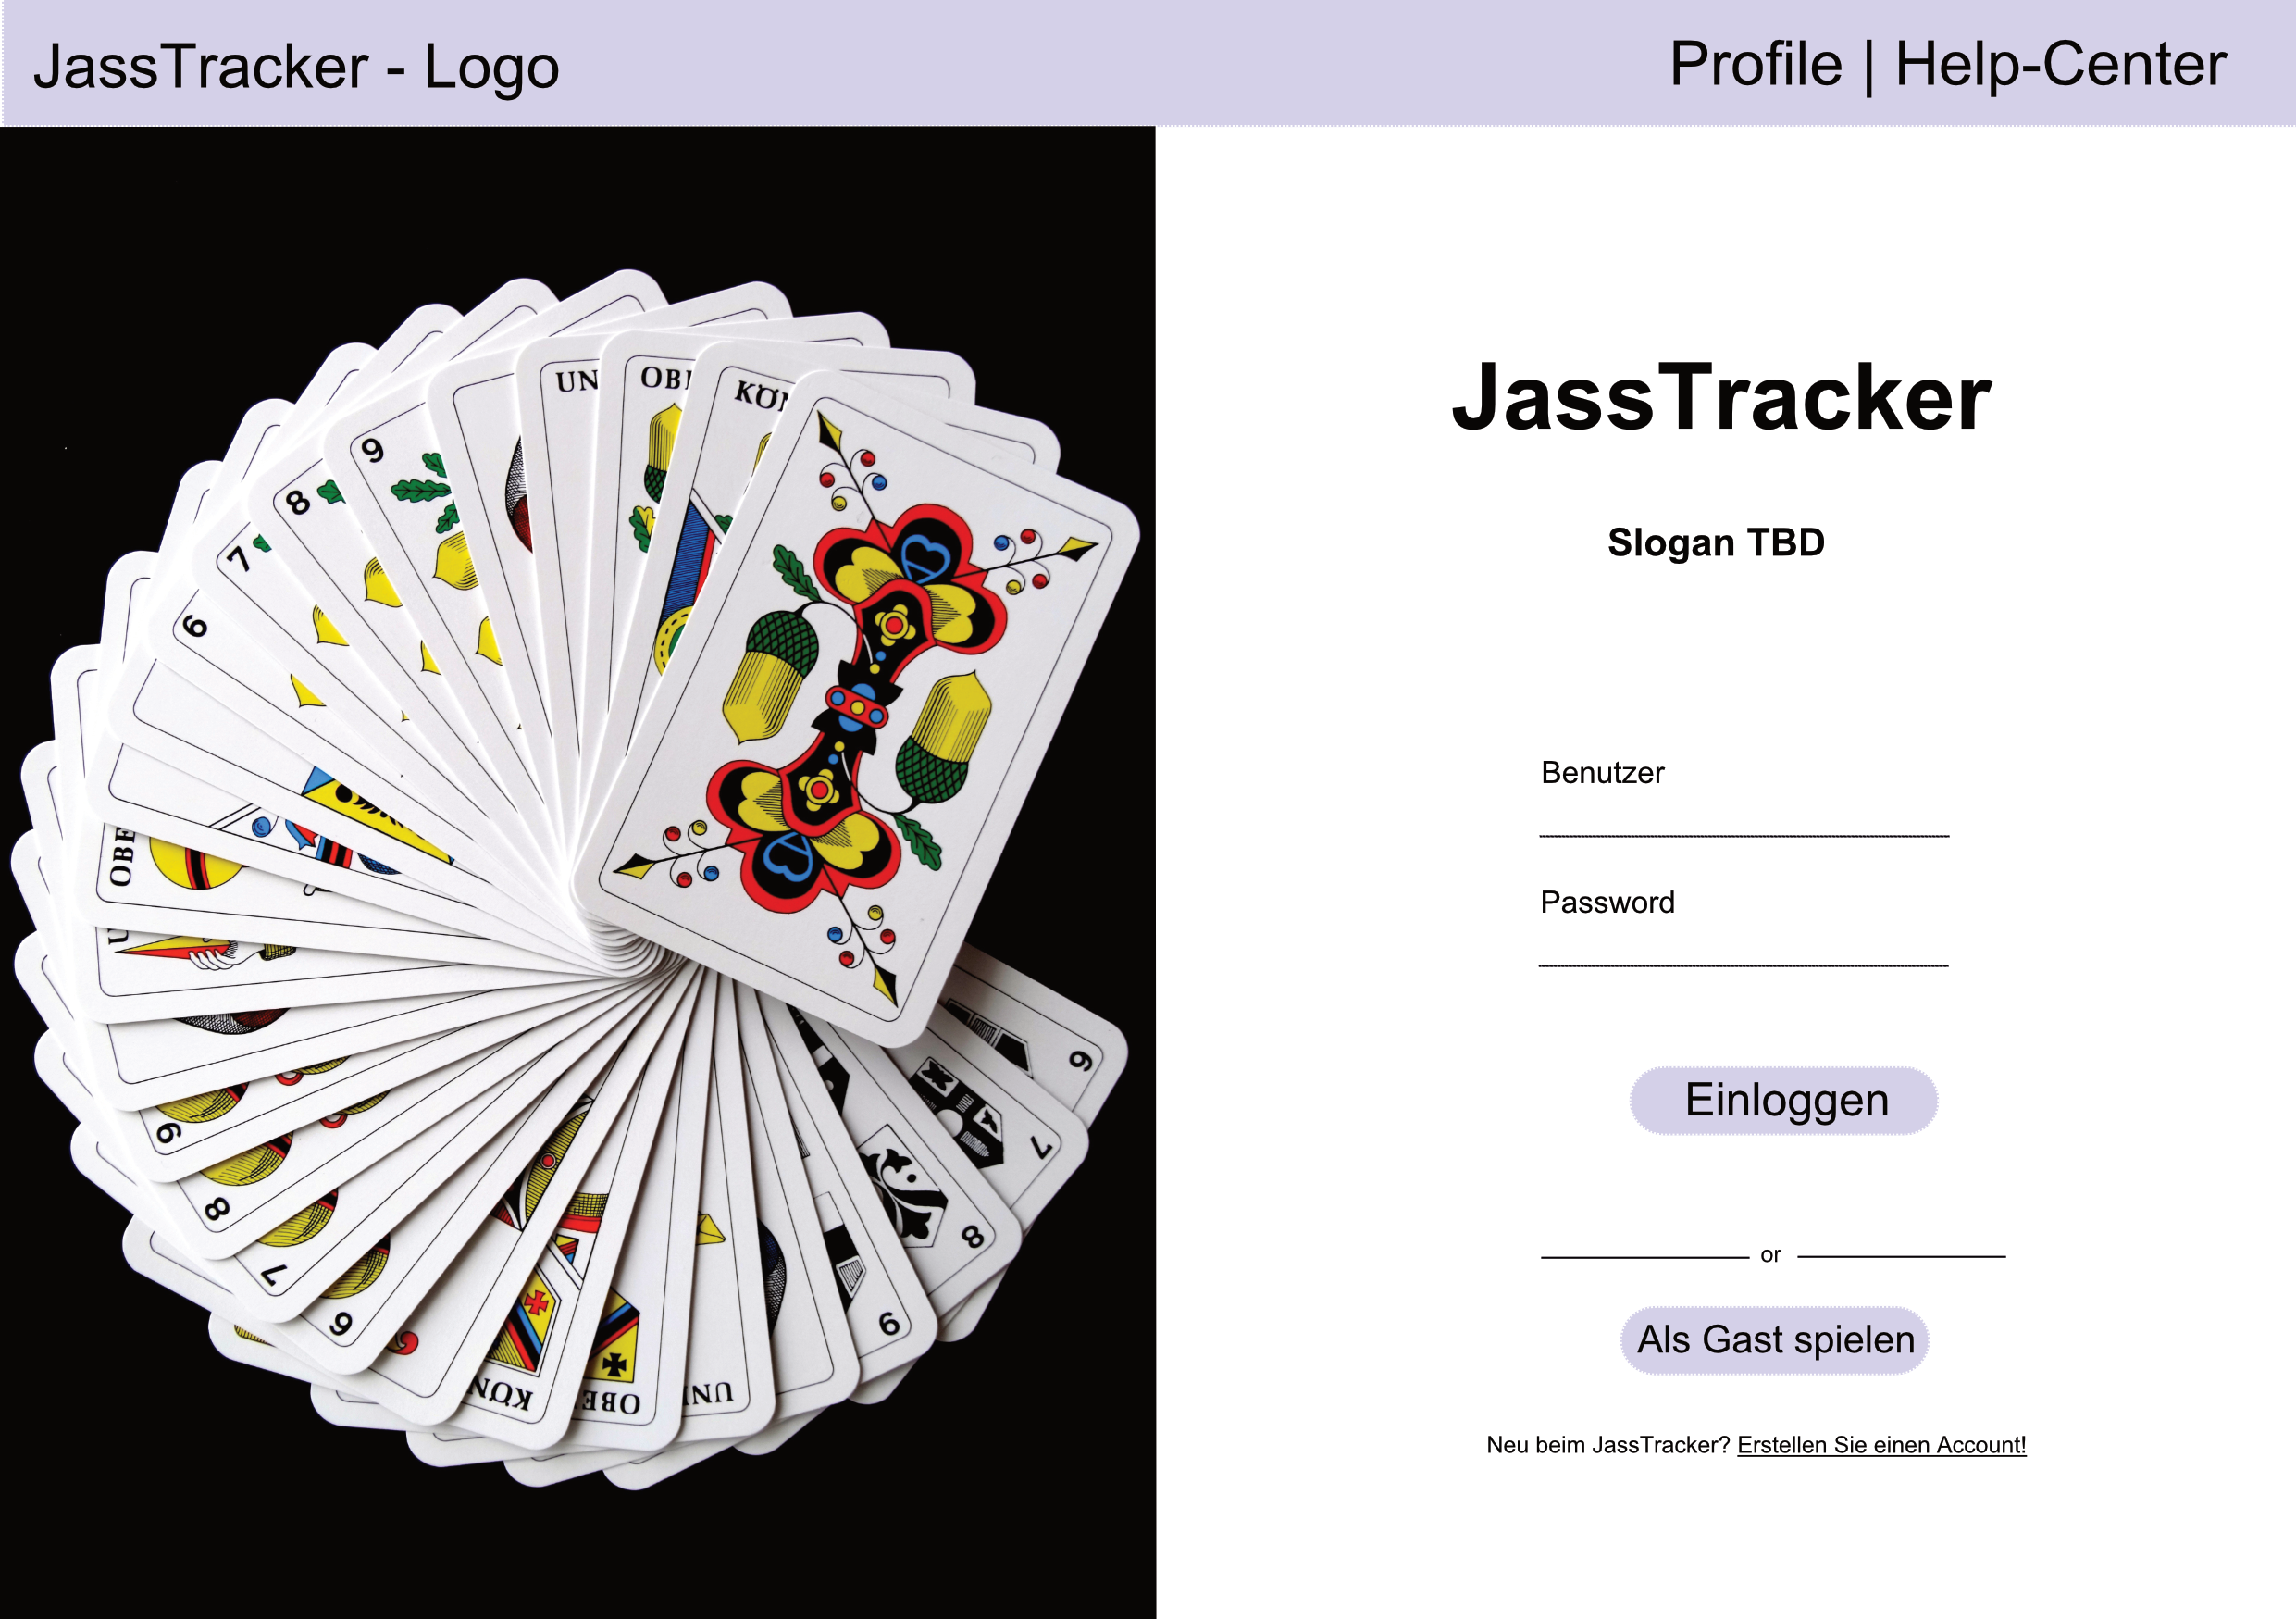
\includegraphics[height=10cm, width=\textwidth]{resources/mockups/mockup-login.png}
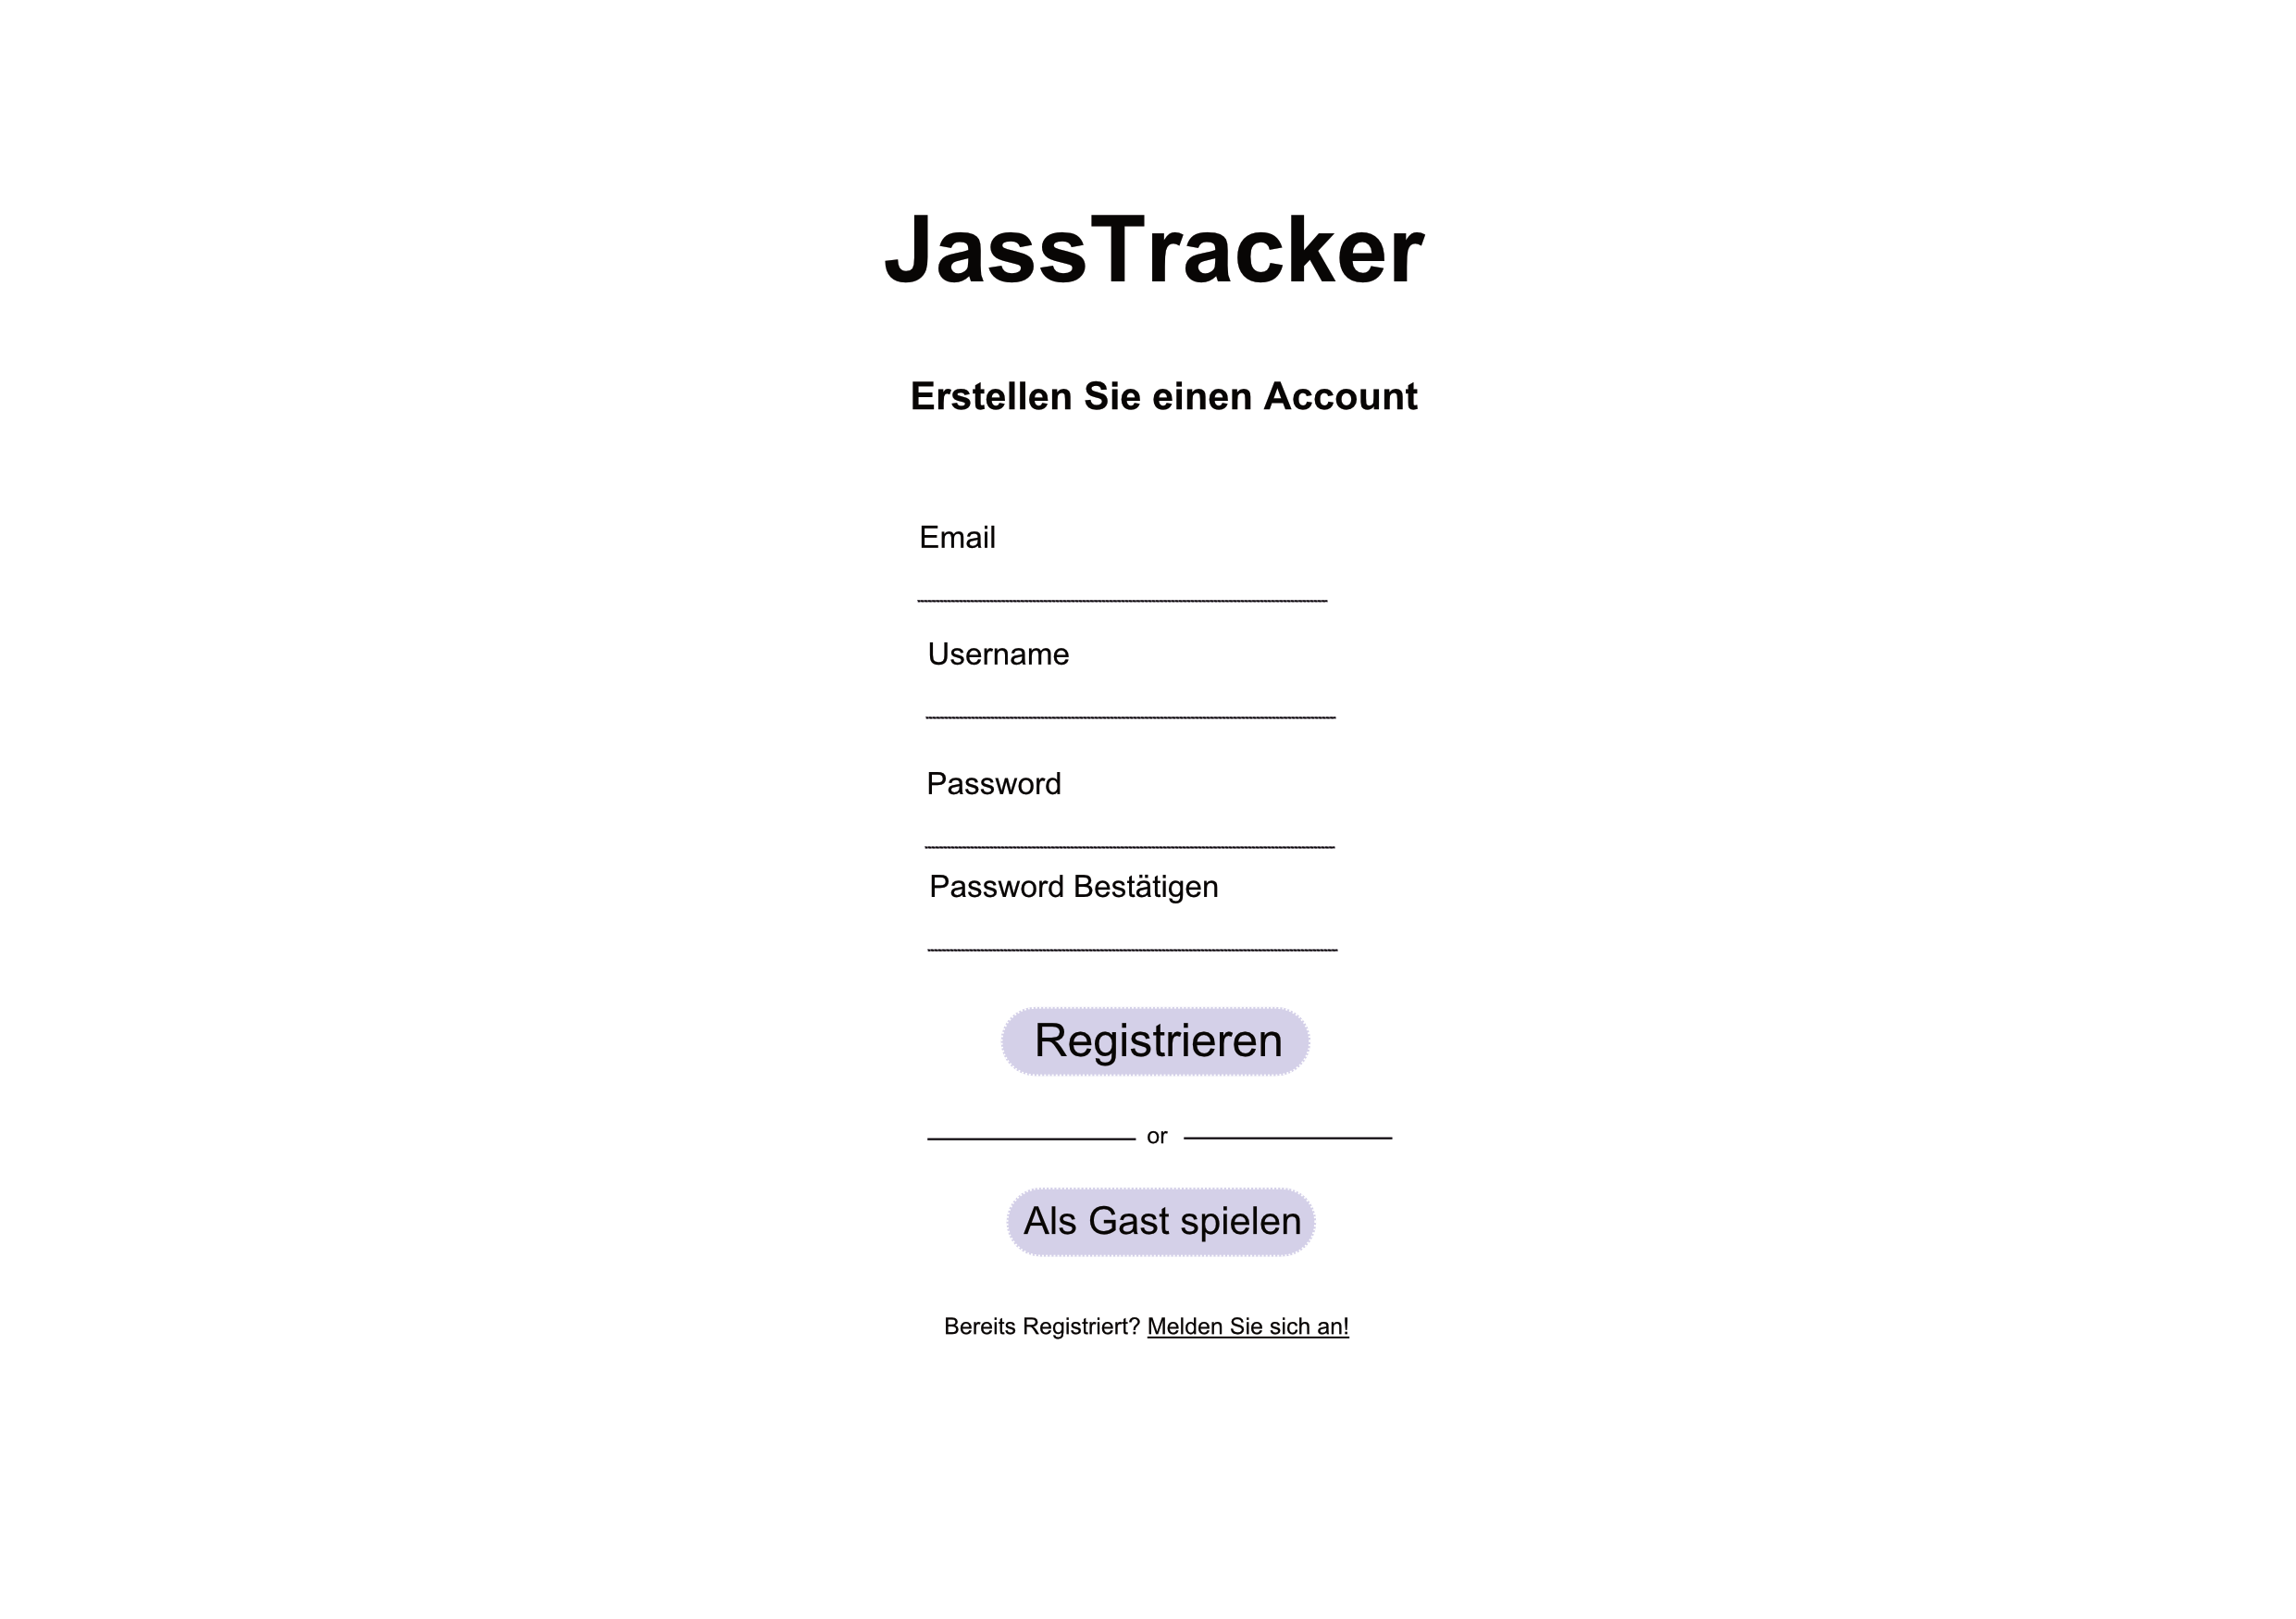
\includegraphics[height=10cm, width=\textwidth]{resources/mockups/mockup-register.png}
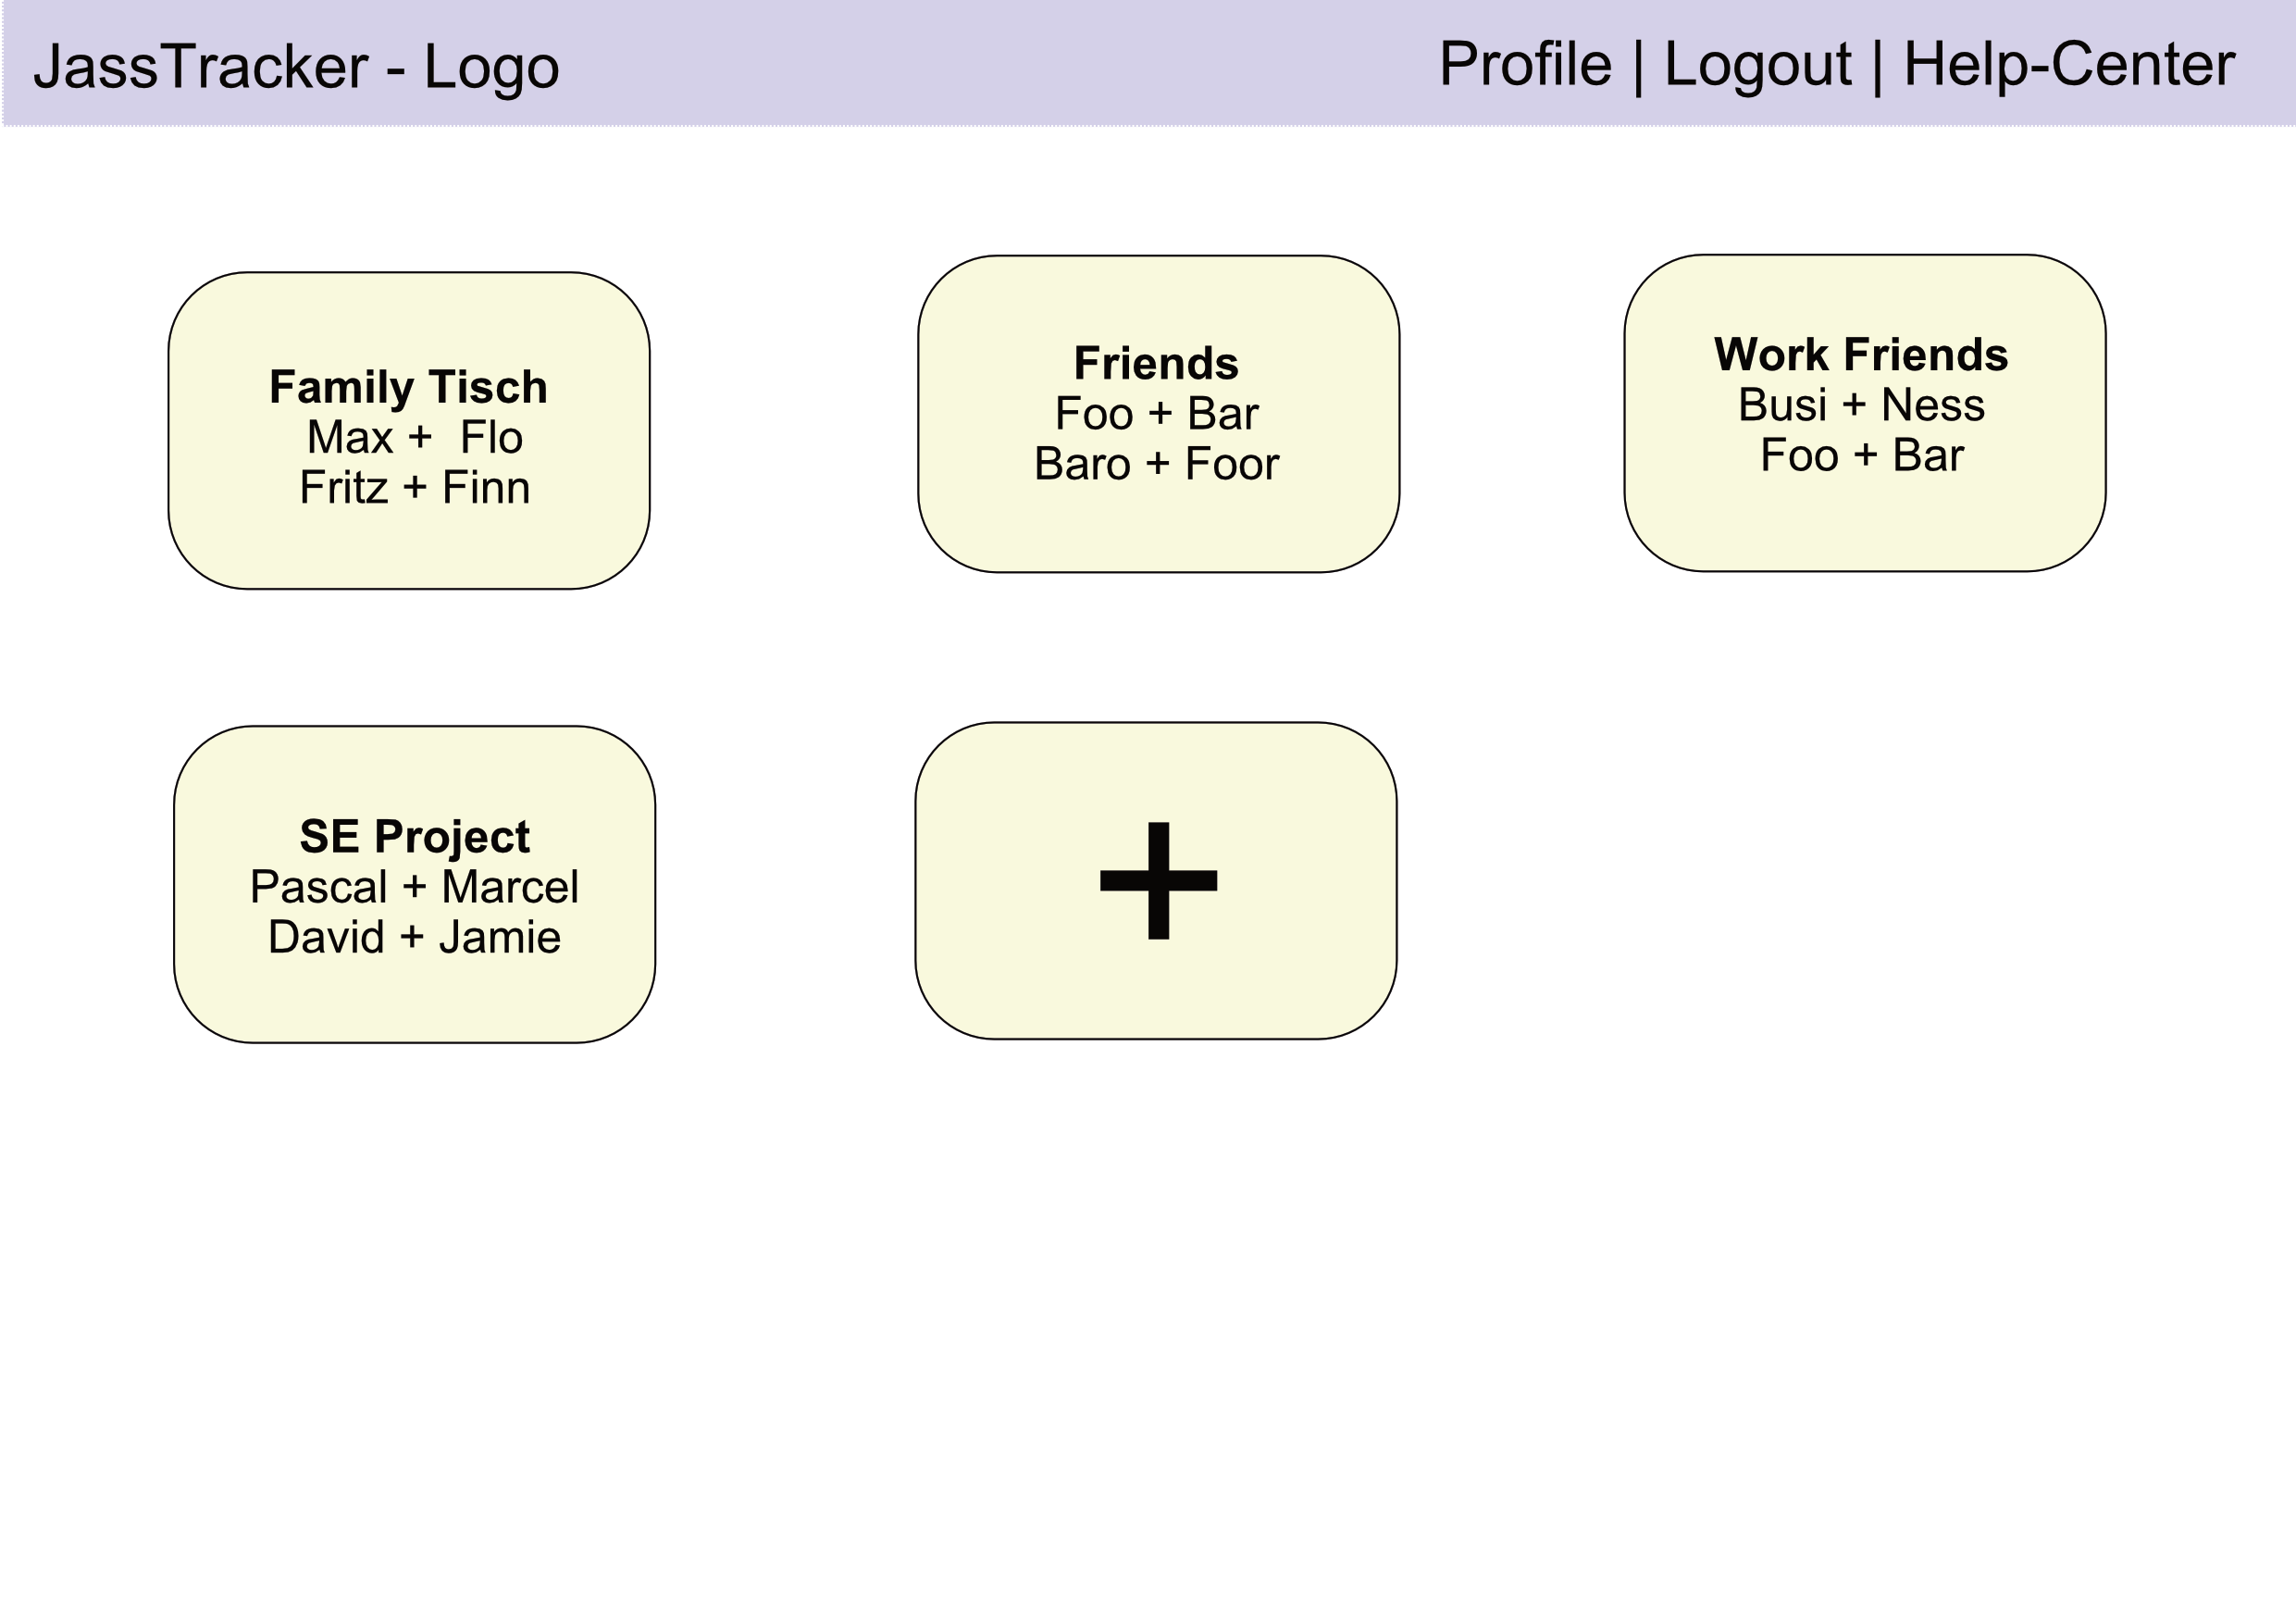
\includegraphics[height=10cm, width=\textwidth]{resources/mockups/mockup-table-overview.png}
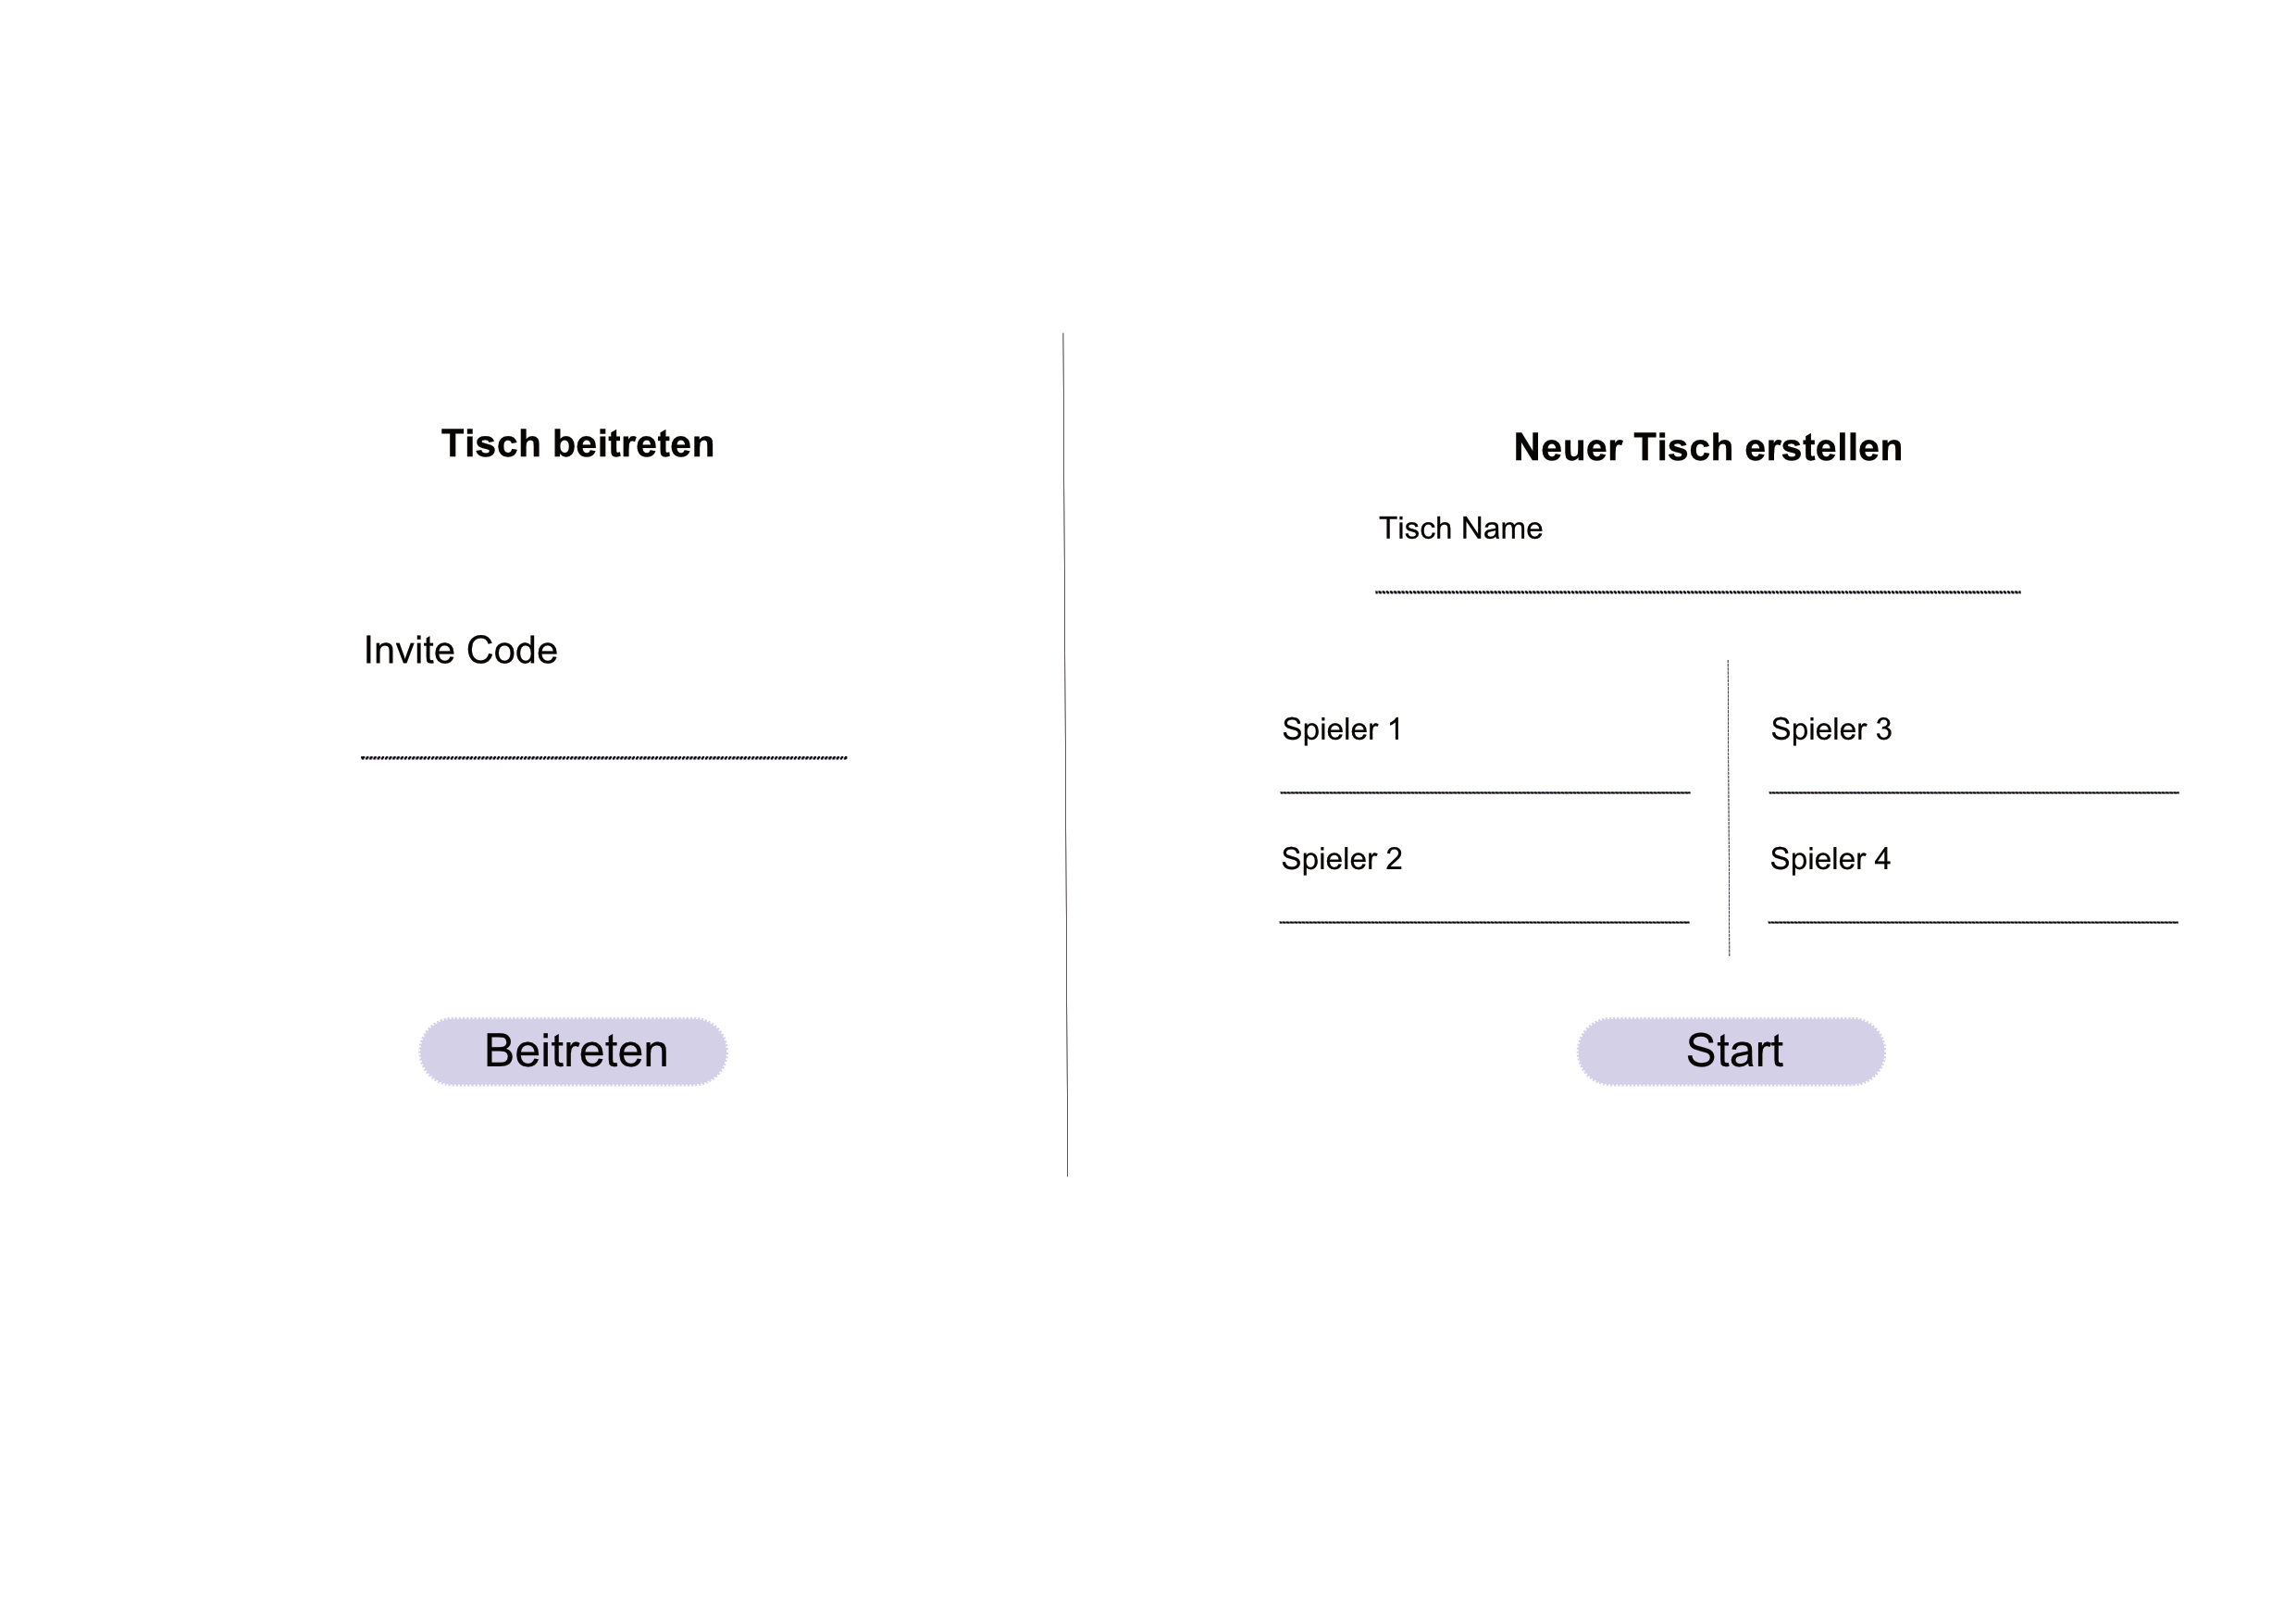
\includegraphics[height=10cm, width=\textwidth]{resources/mockups/mockup-create-new-table.png}
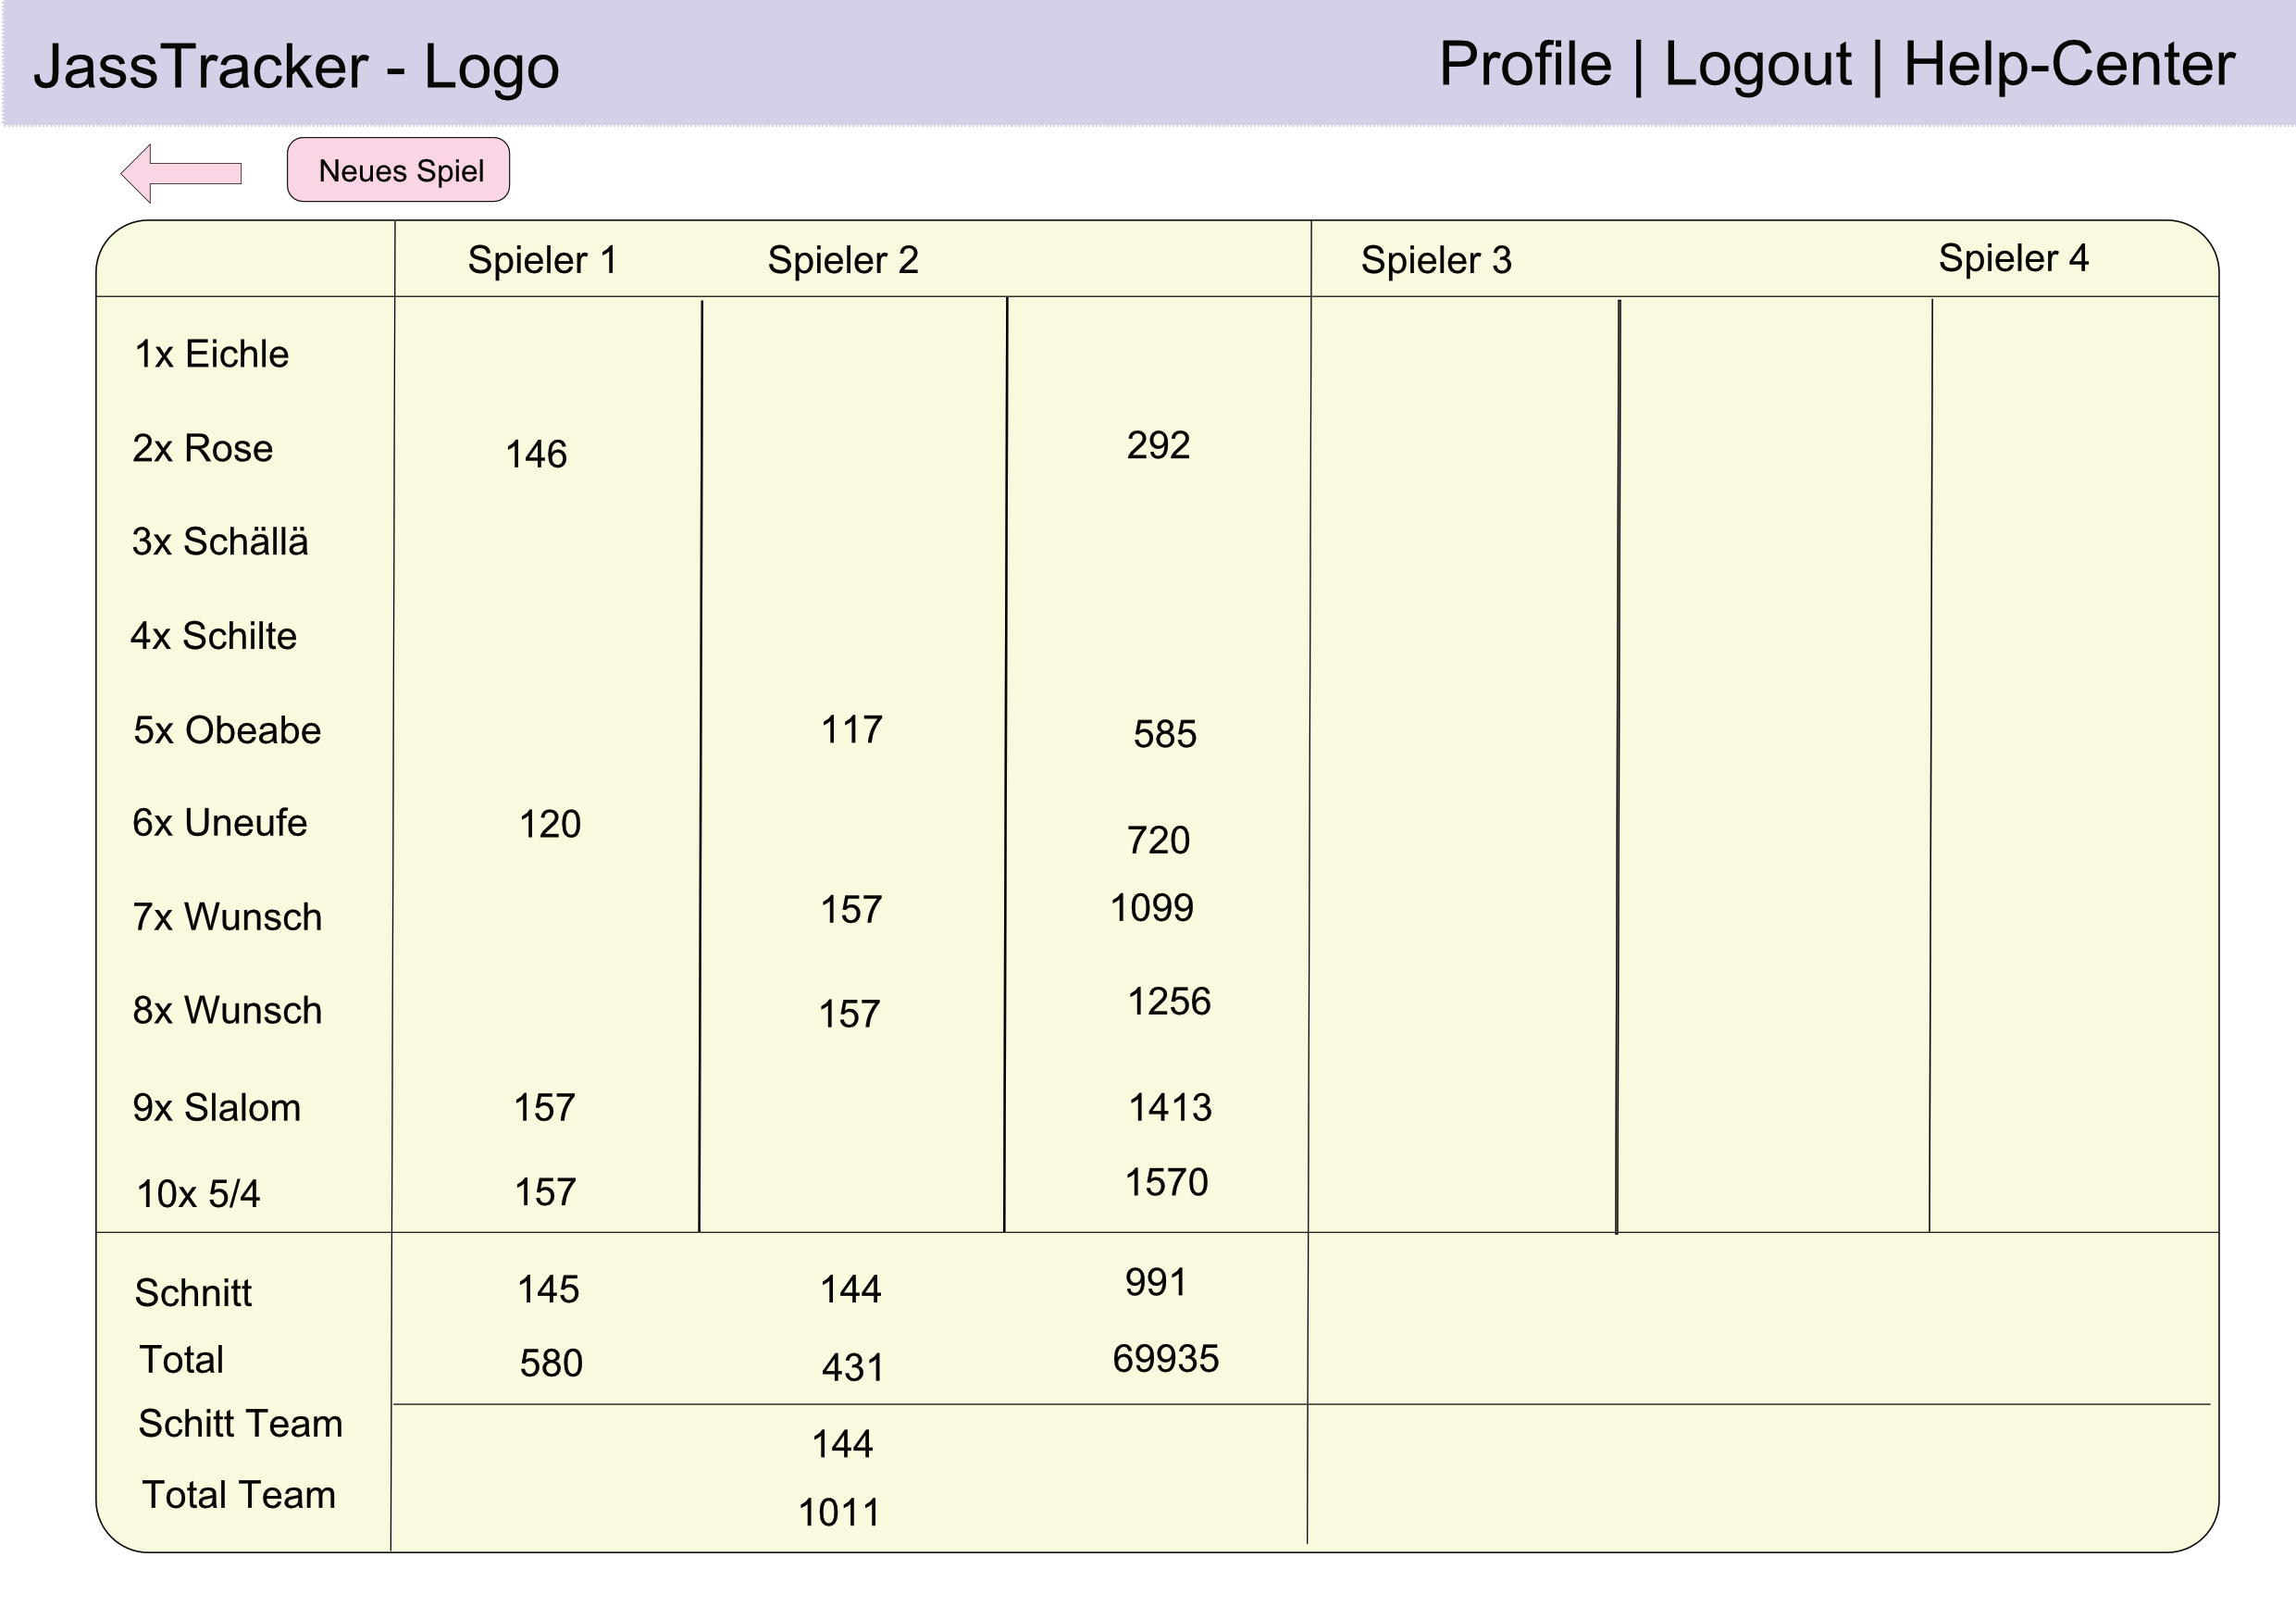
\includegraphics[height=10cm, width=\textwidth]{resources/mockups/mockup-scoreboard.png}
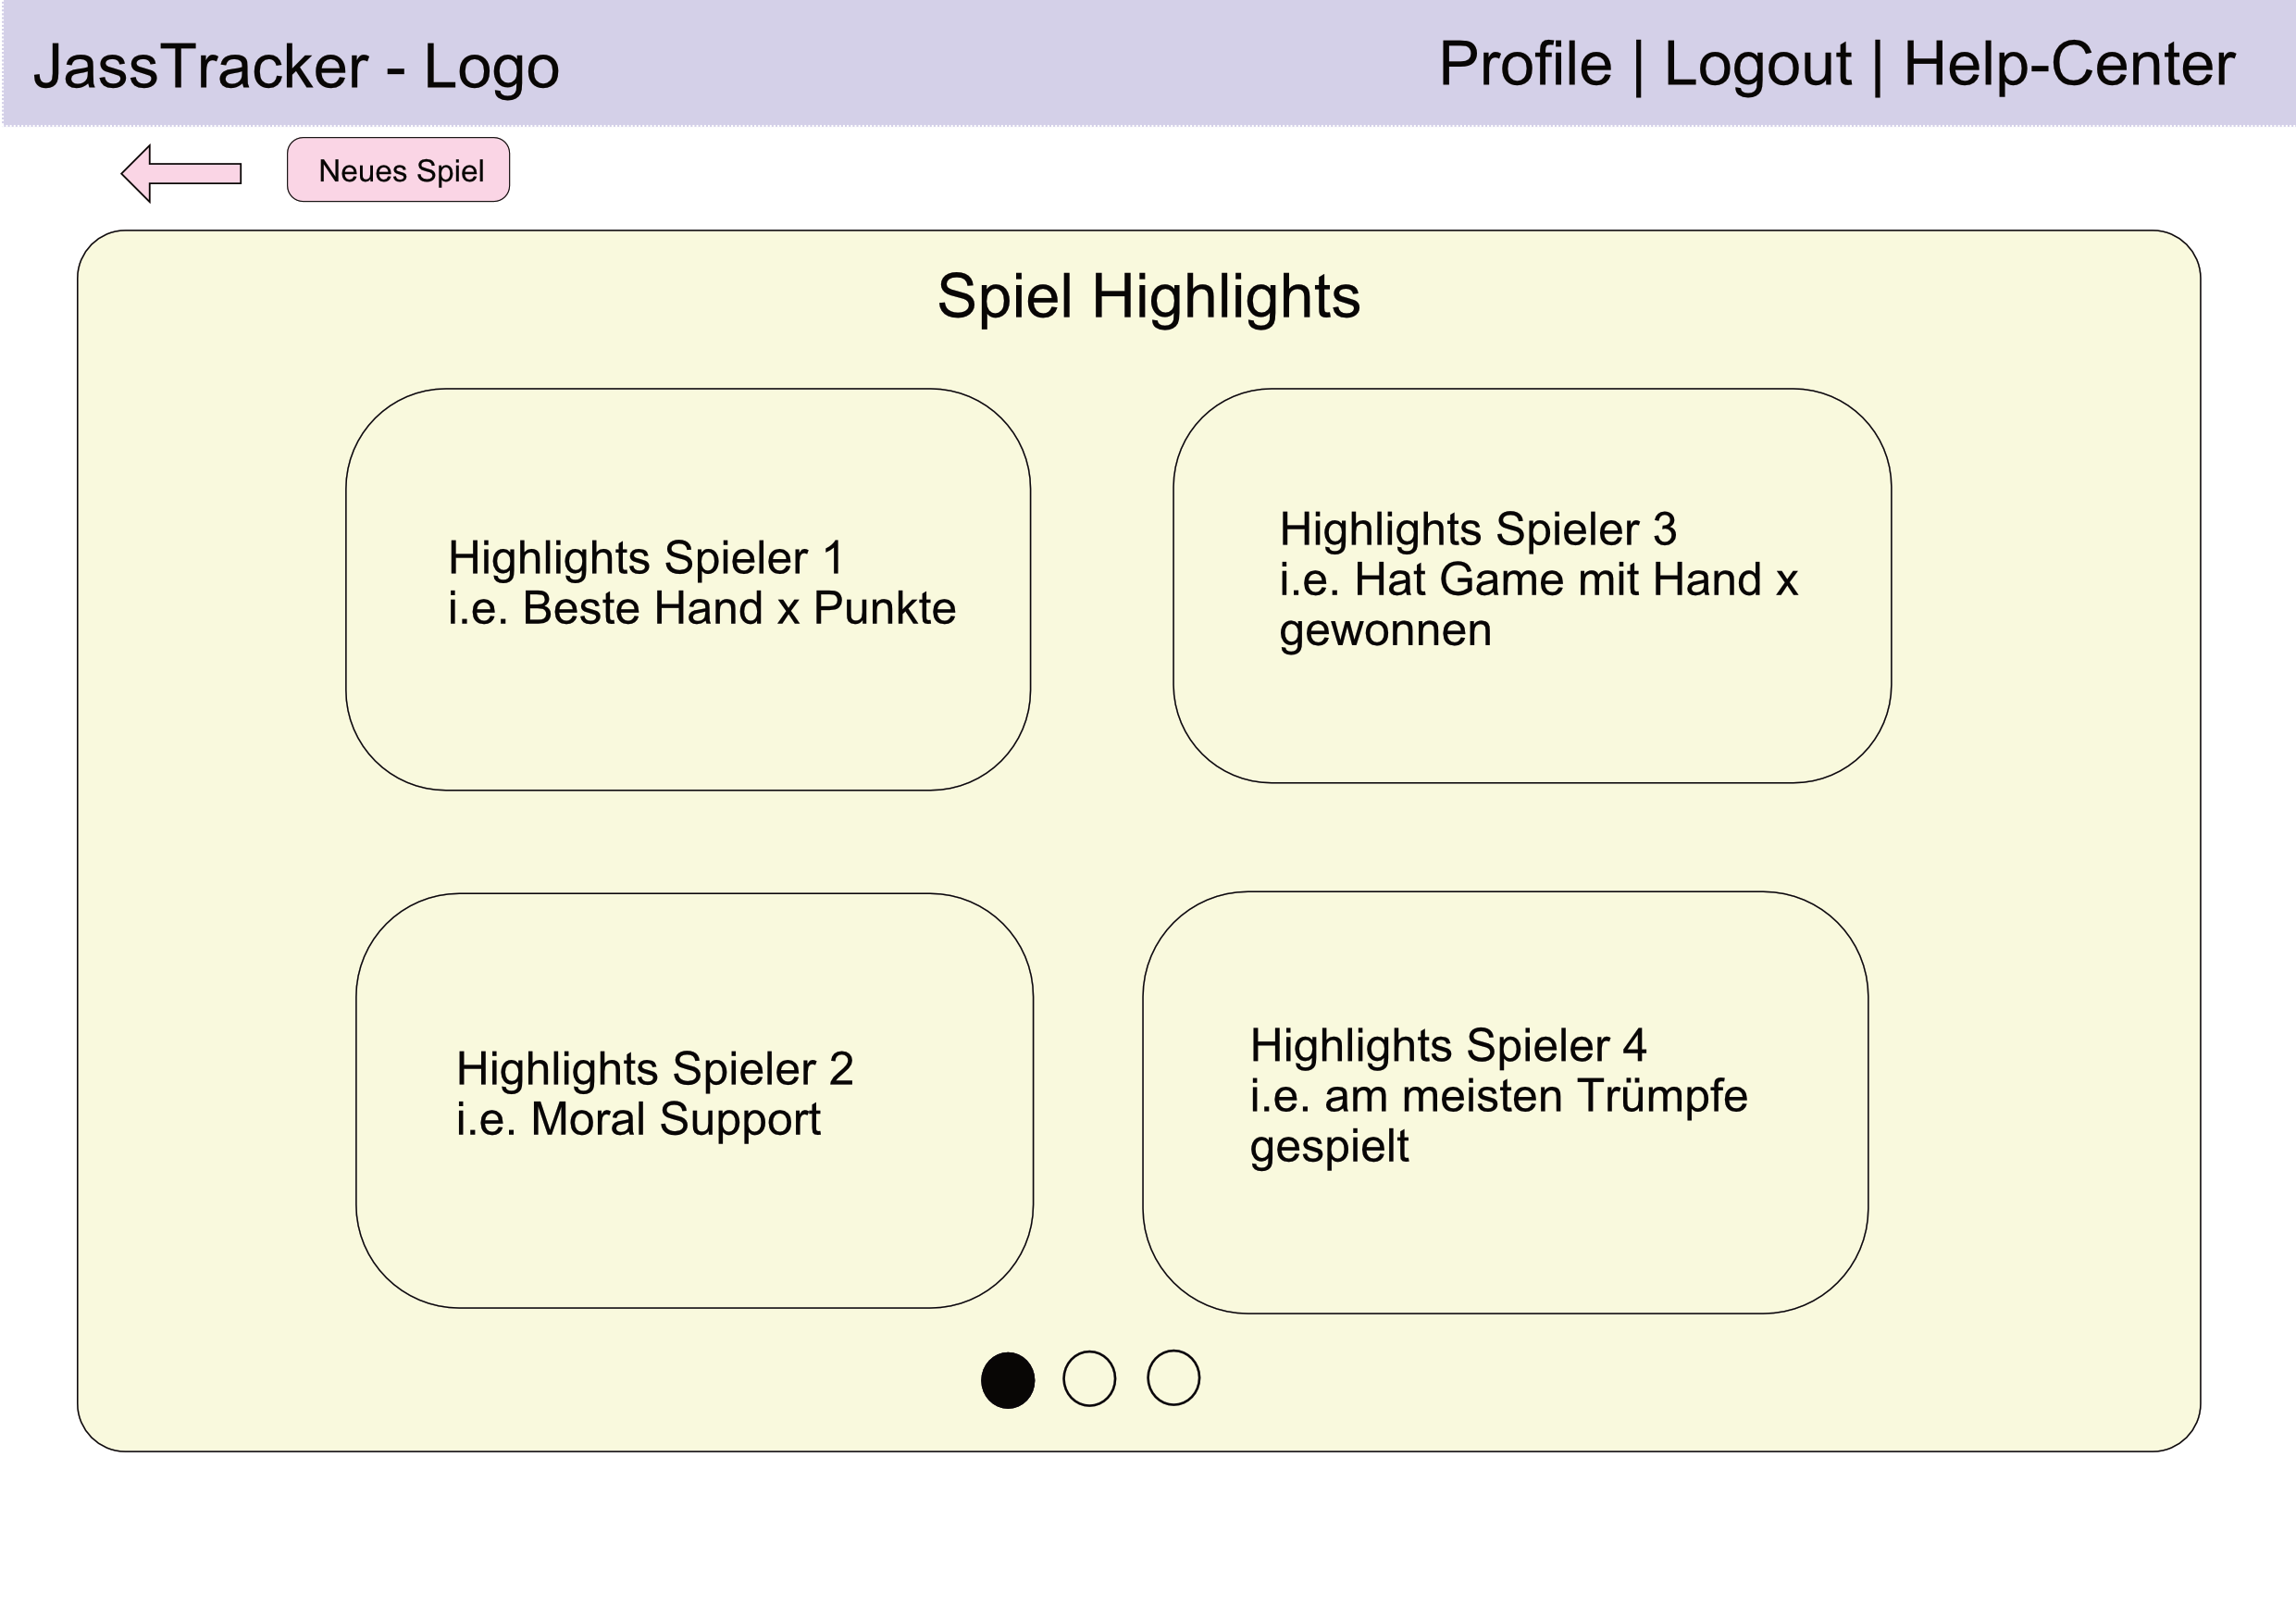
\includegraphics[height=10cm, width=\textwidth]{resources/mockups/mockup-eof-hightlights.png}
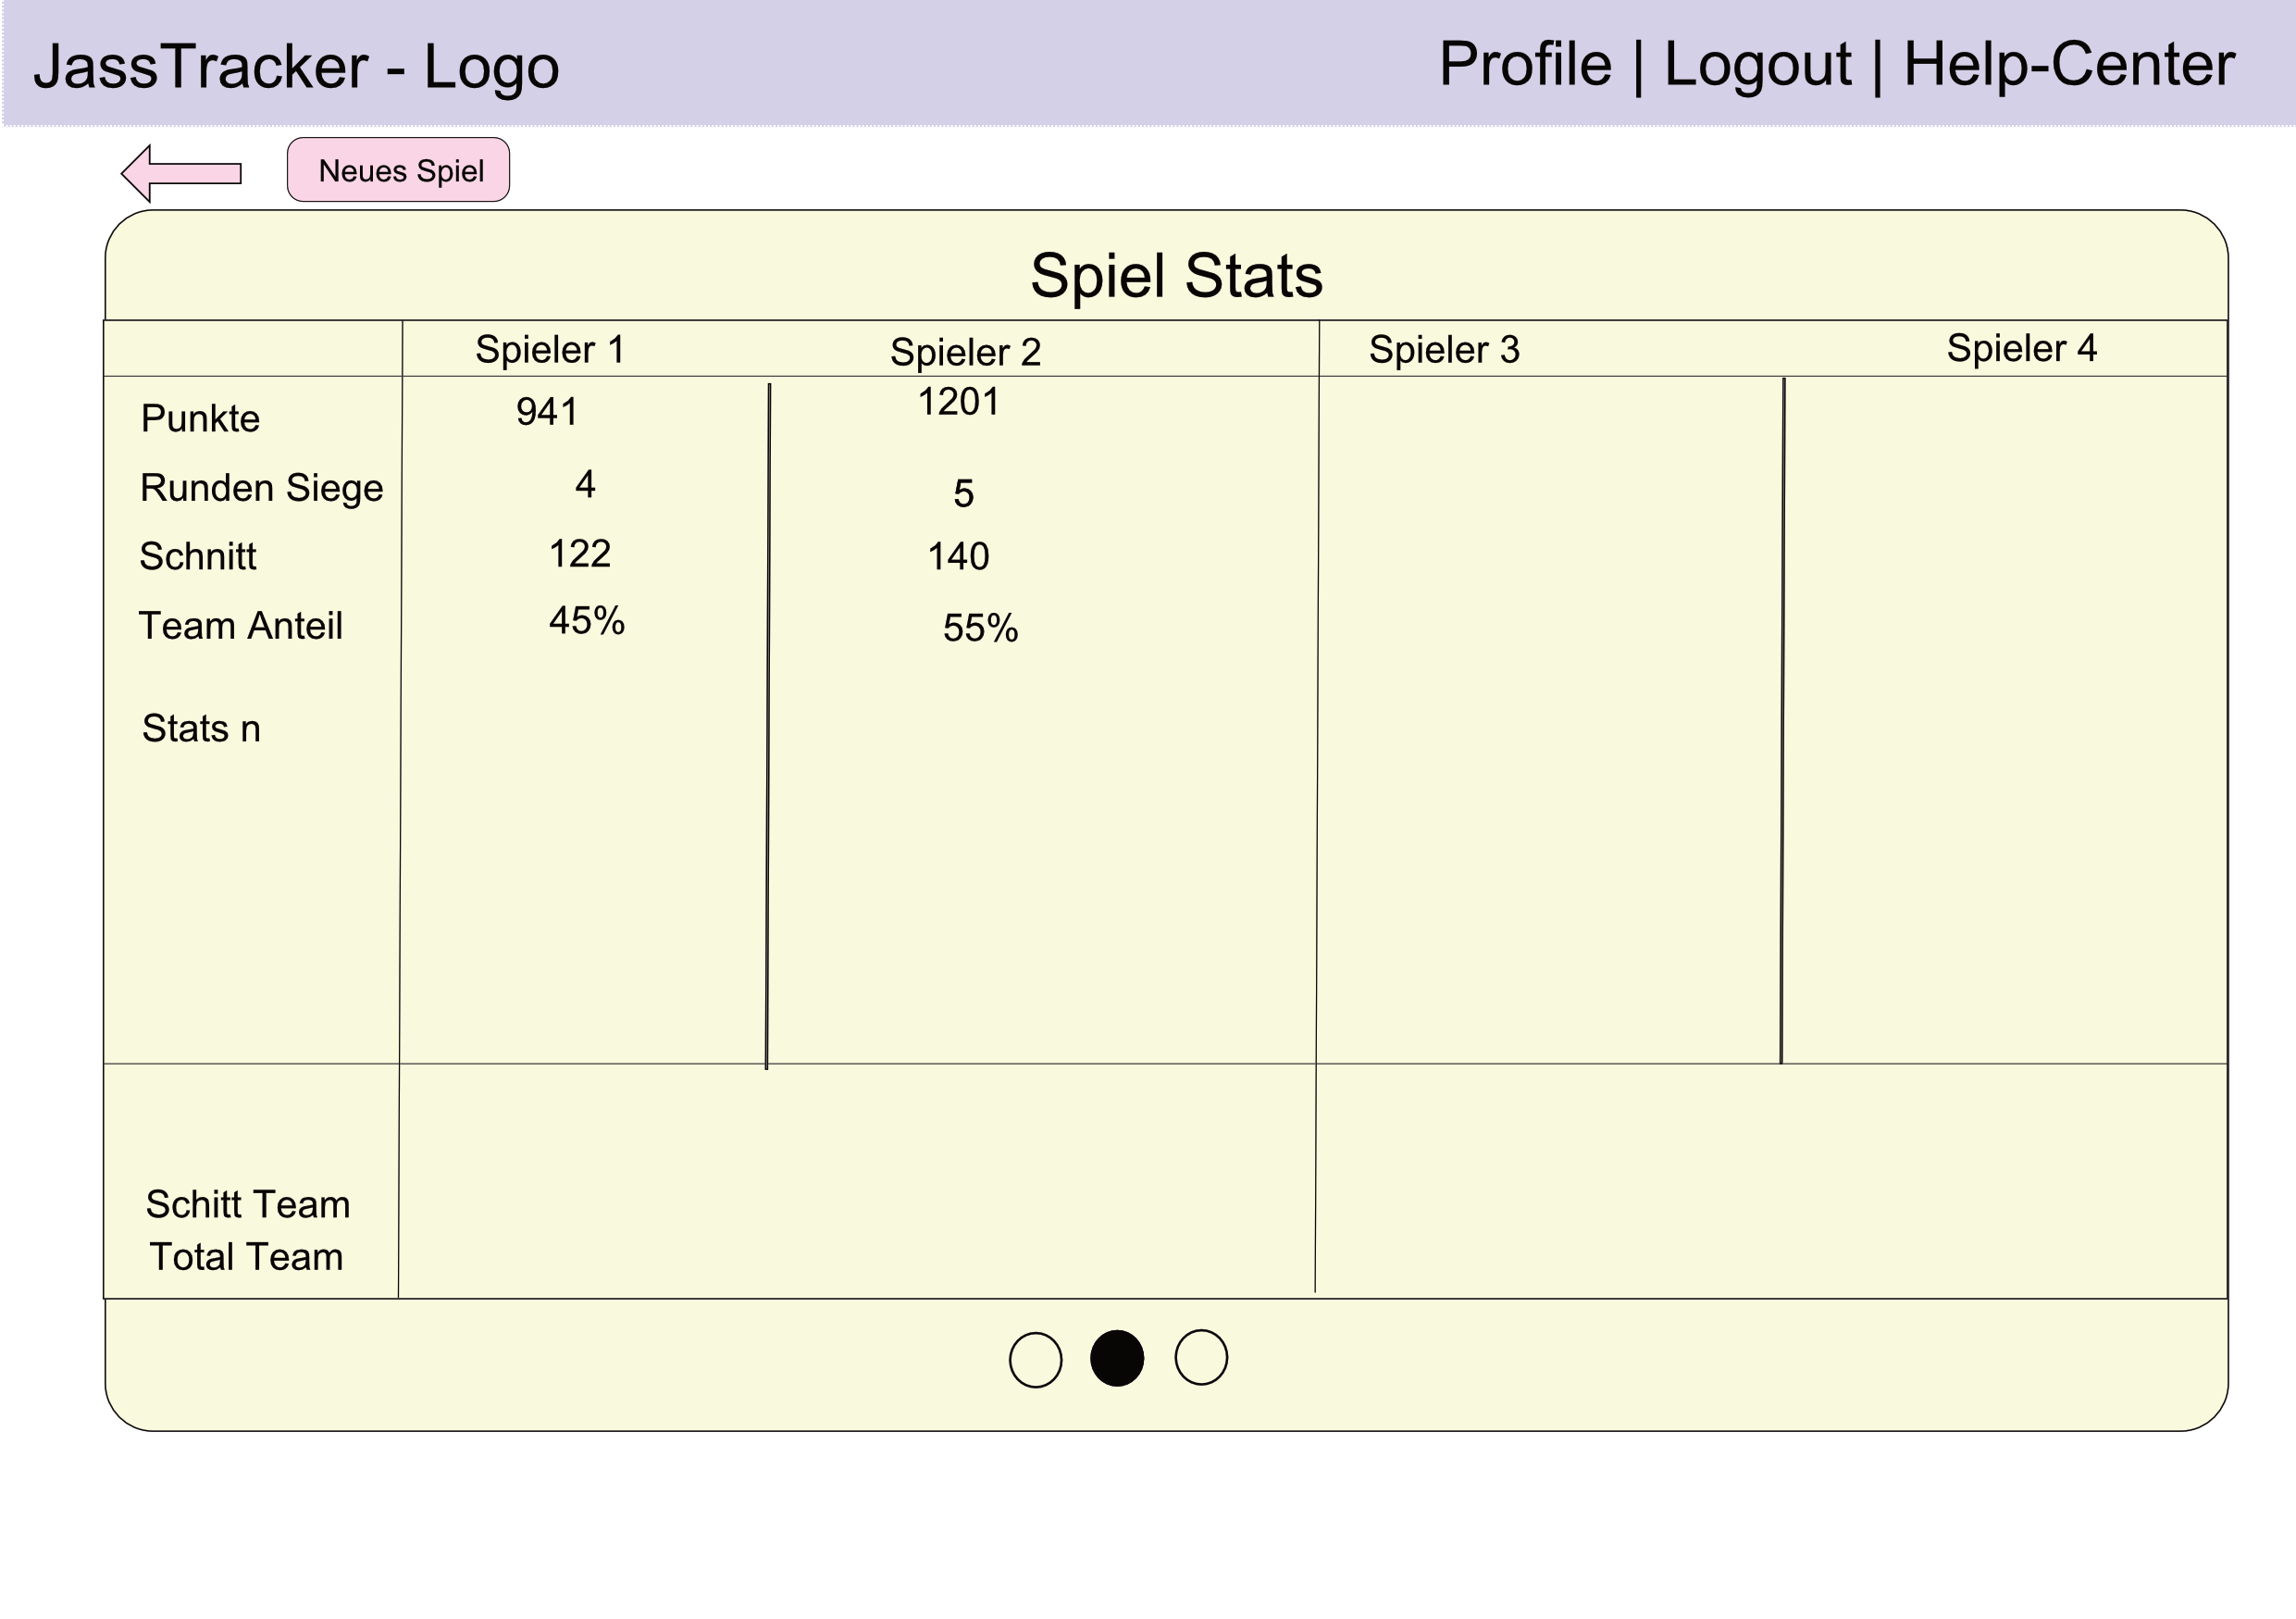
\includegraphics[height=10cm, width=\textwidth]{resources/mockups/mockup-eof-stats.png}
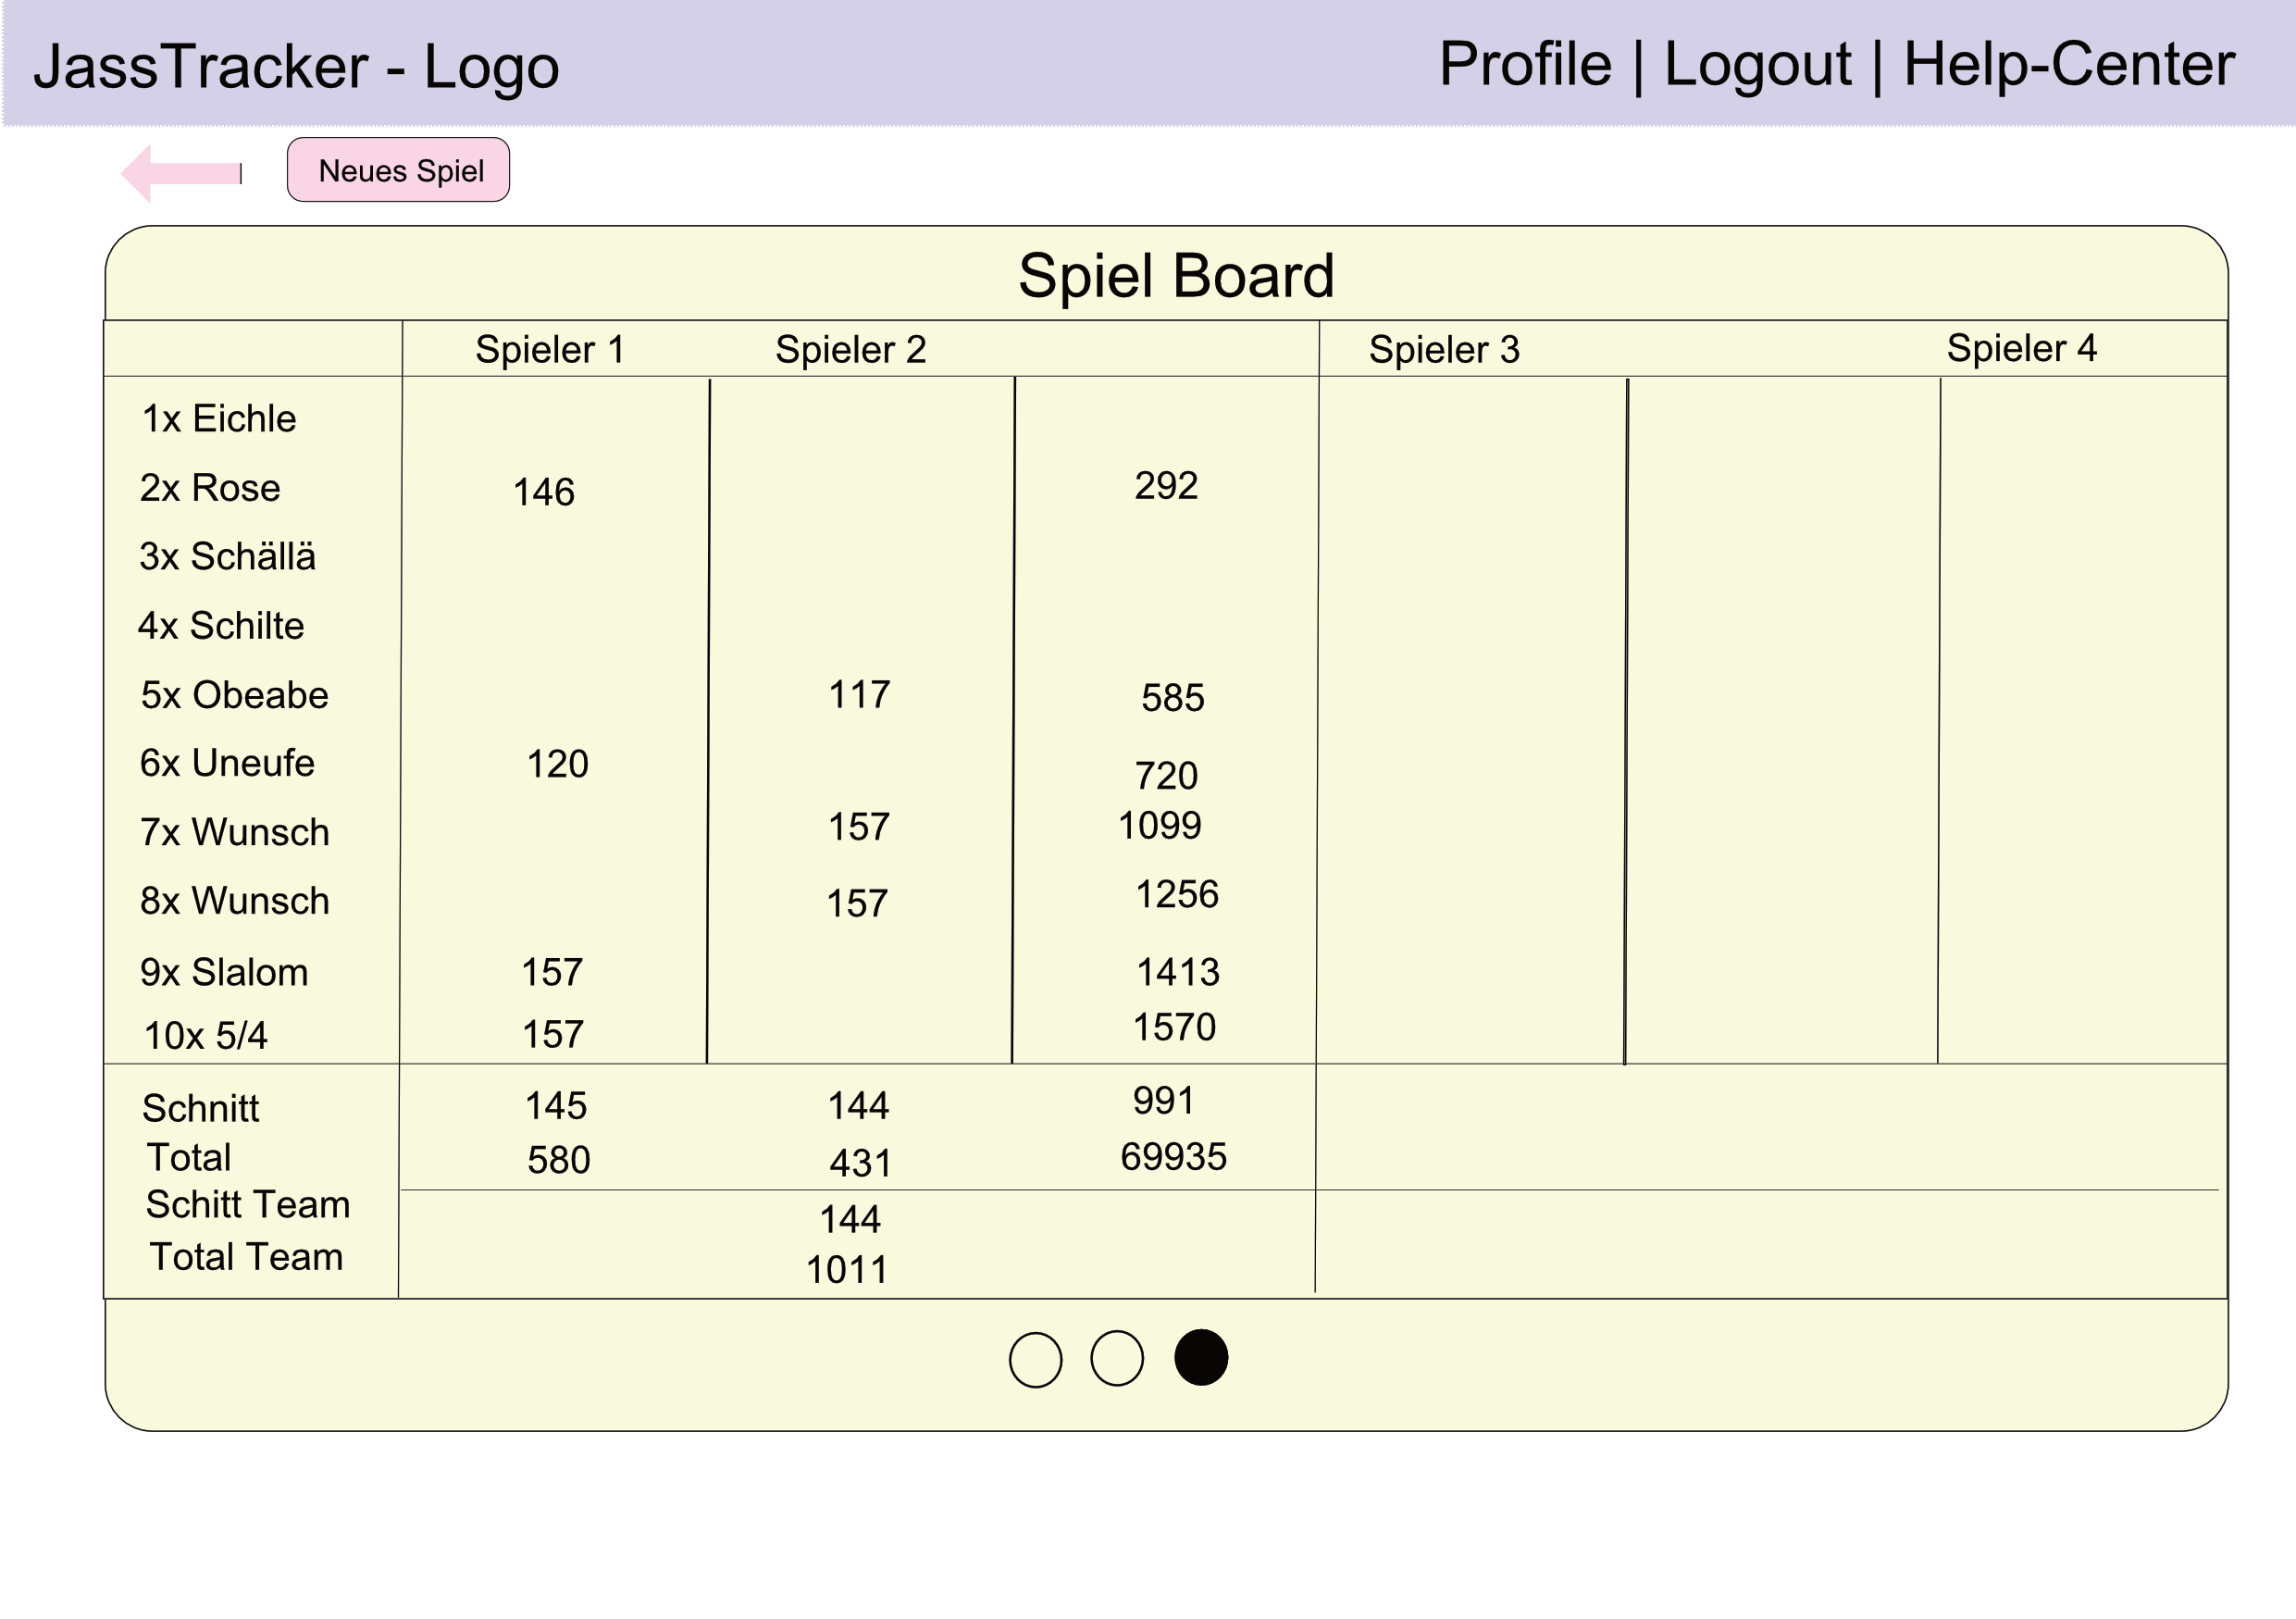
\includegraphics[height=10cm, width=\textwidth]{resources/mockups/mockup-eof-scoreboard.png}
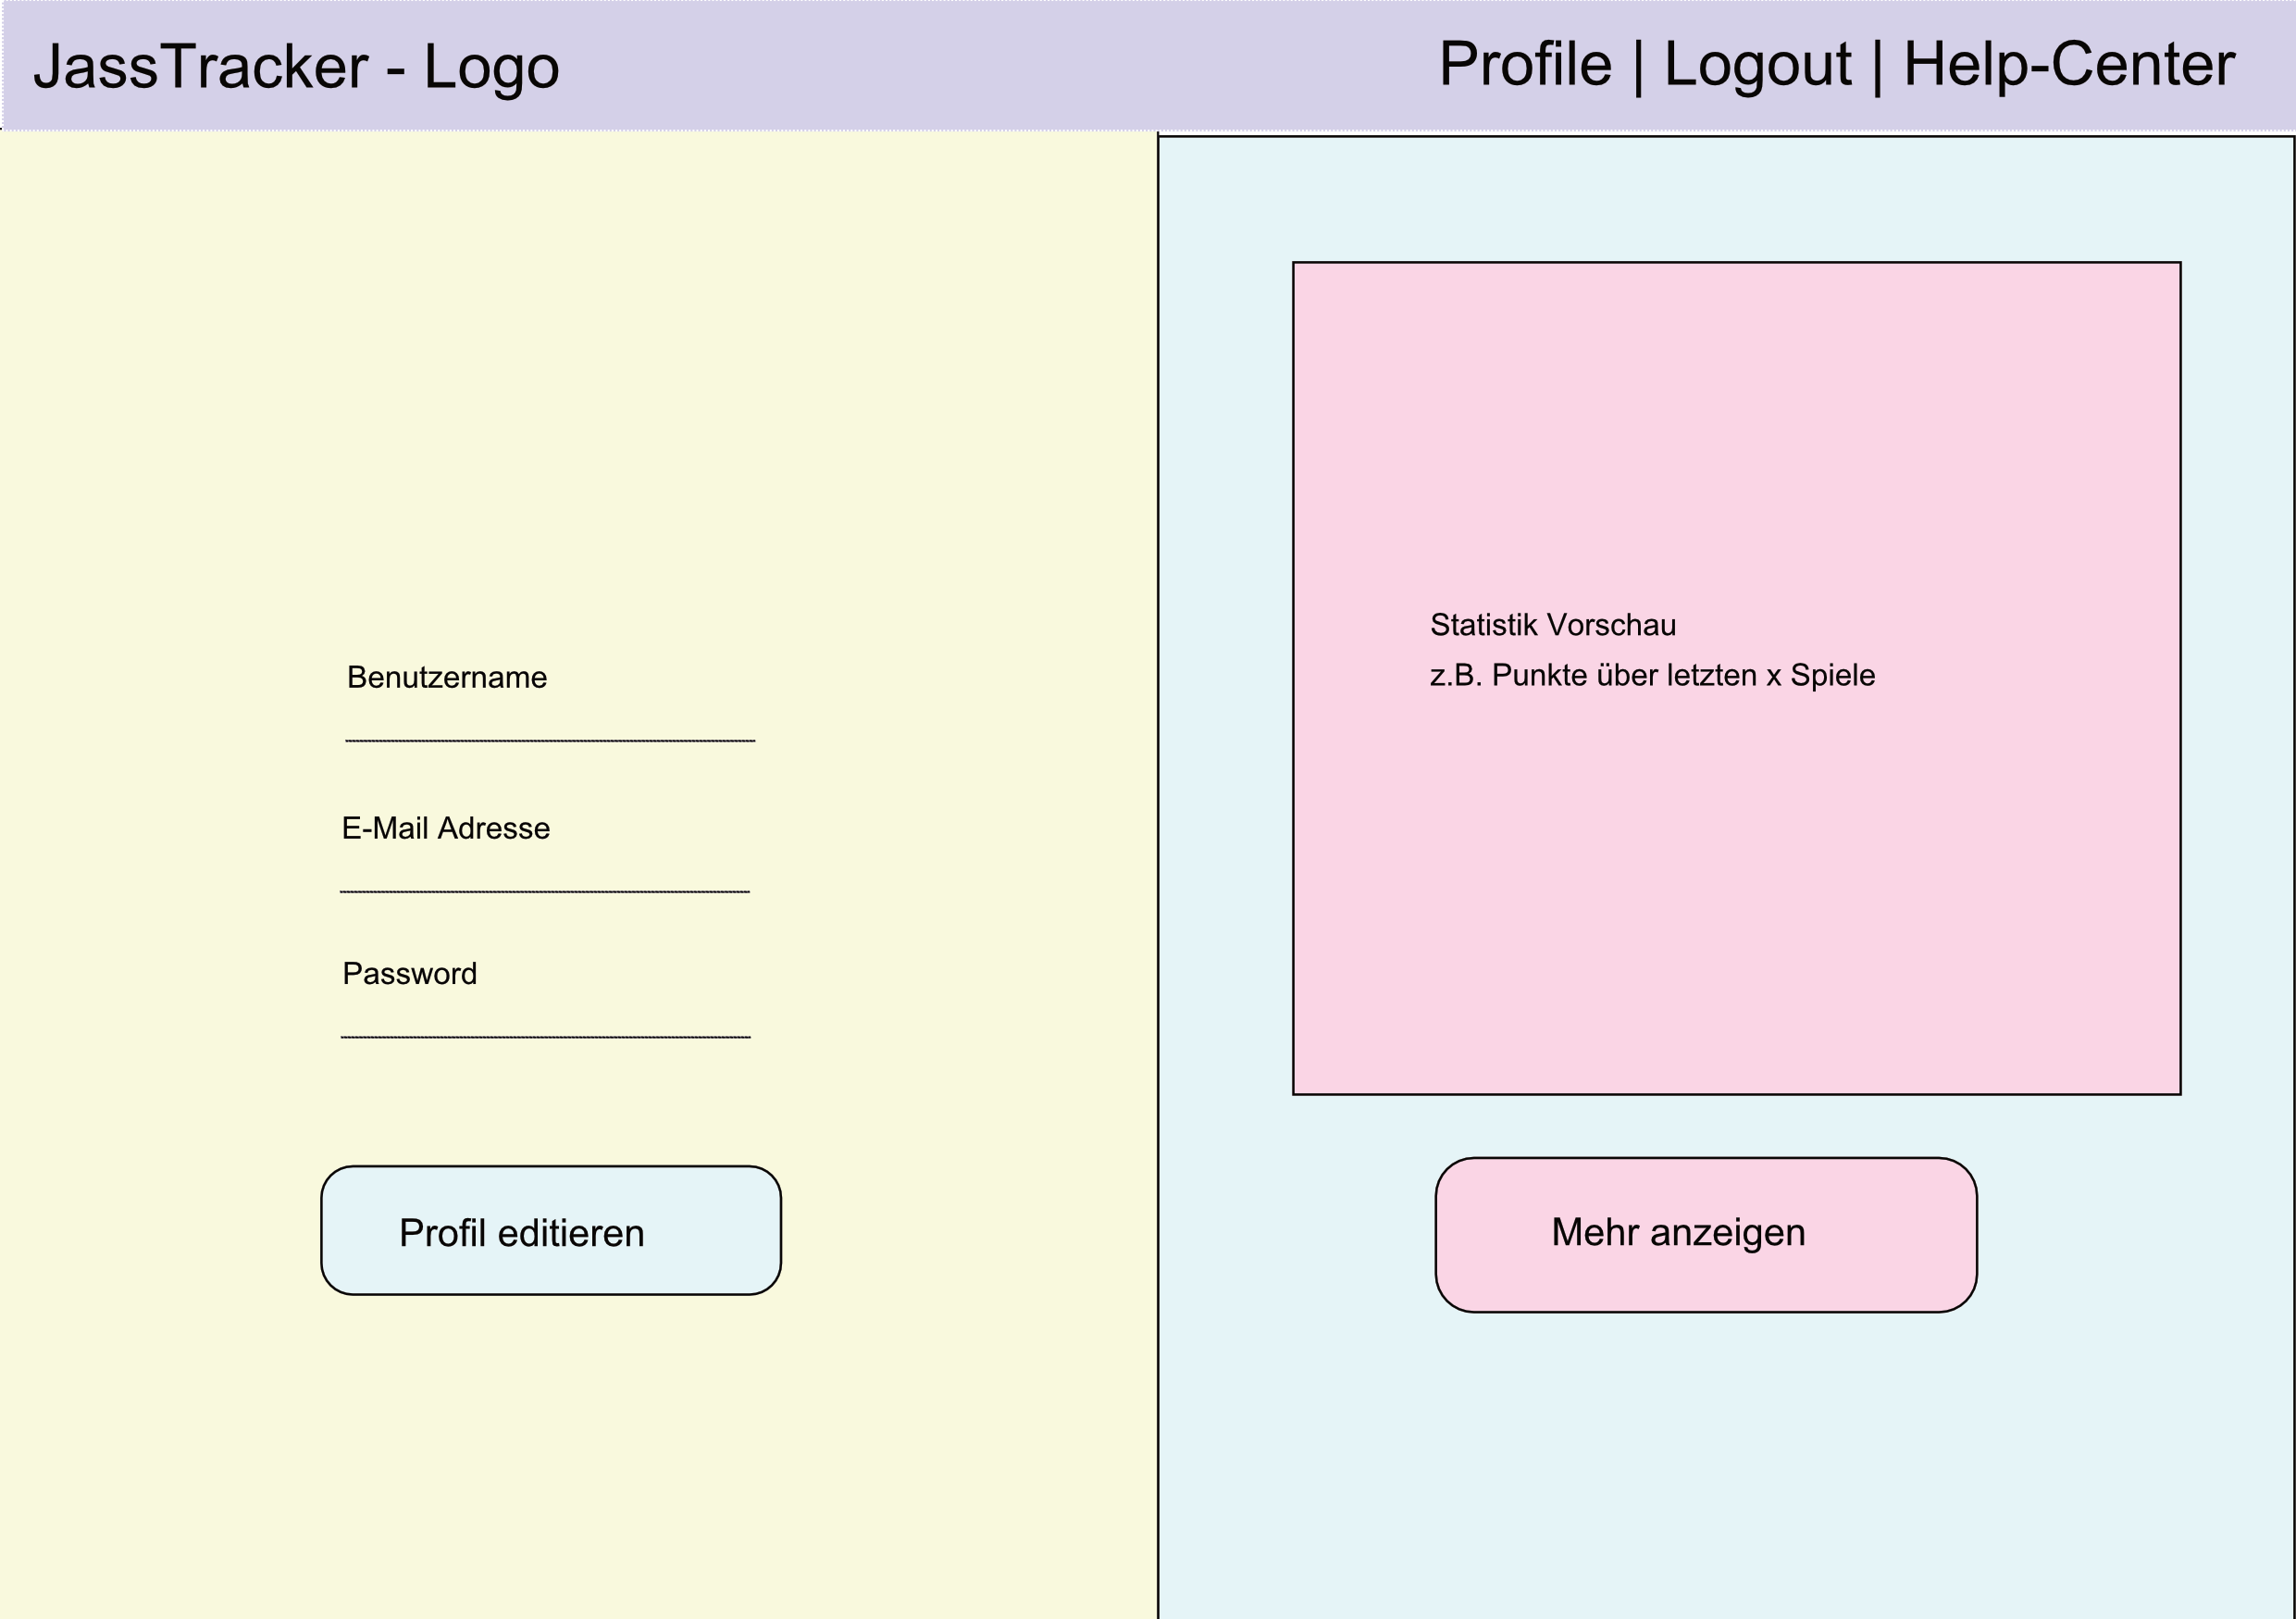
\includegraphics[height=10cm, width=\textwidth]{resources/mockups/mockup-profile-overview.png}
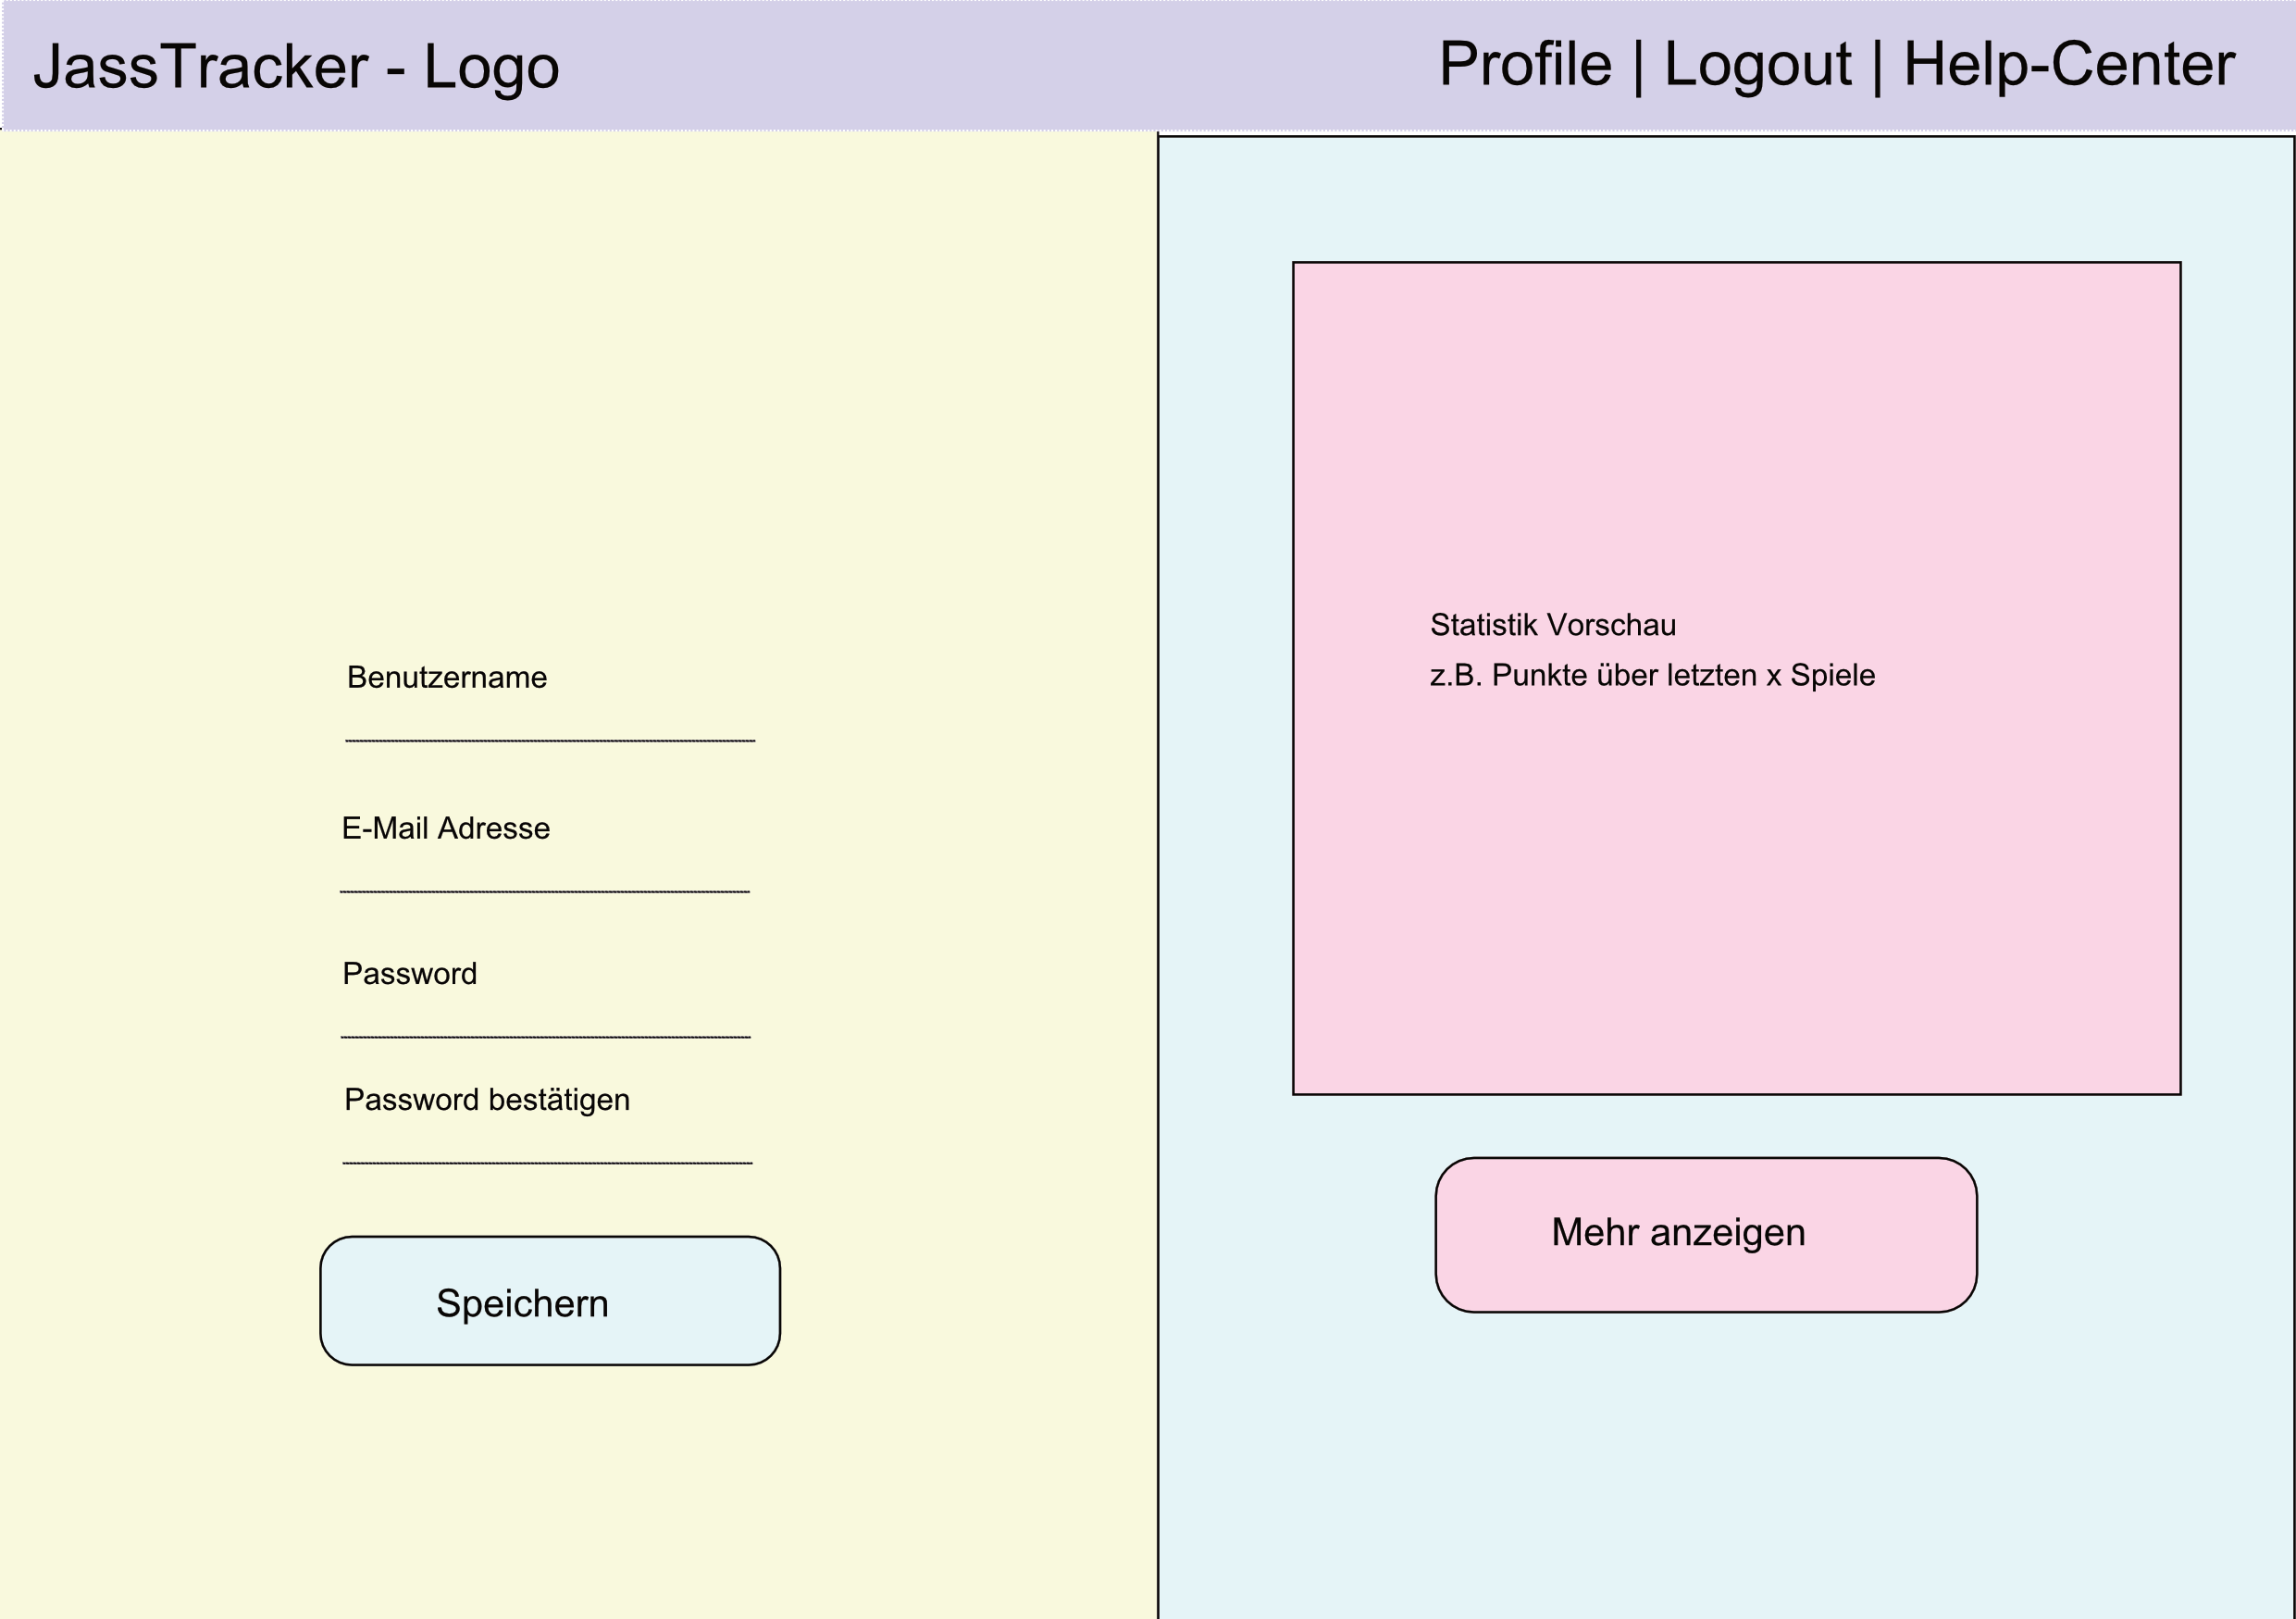
\includegraphics[height=10cm, width=\textwidth]{resources/mockups/mockup-profile-overview-edit.png}
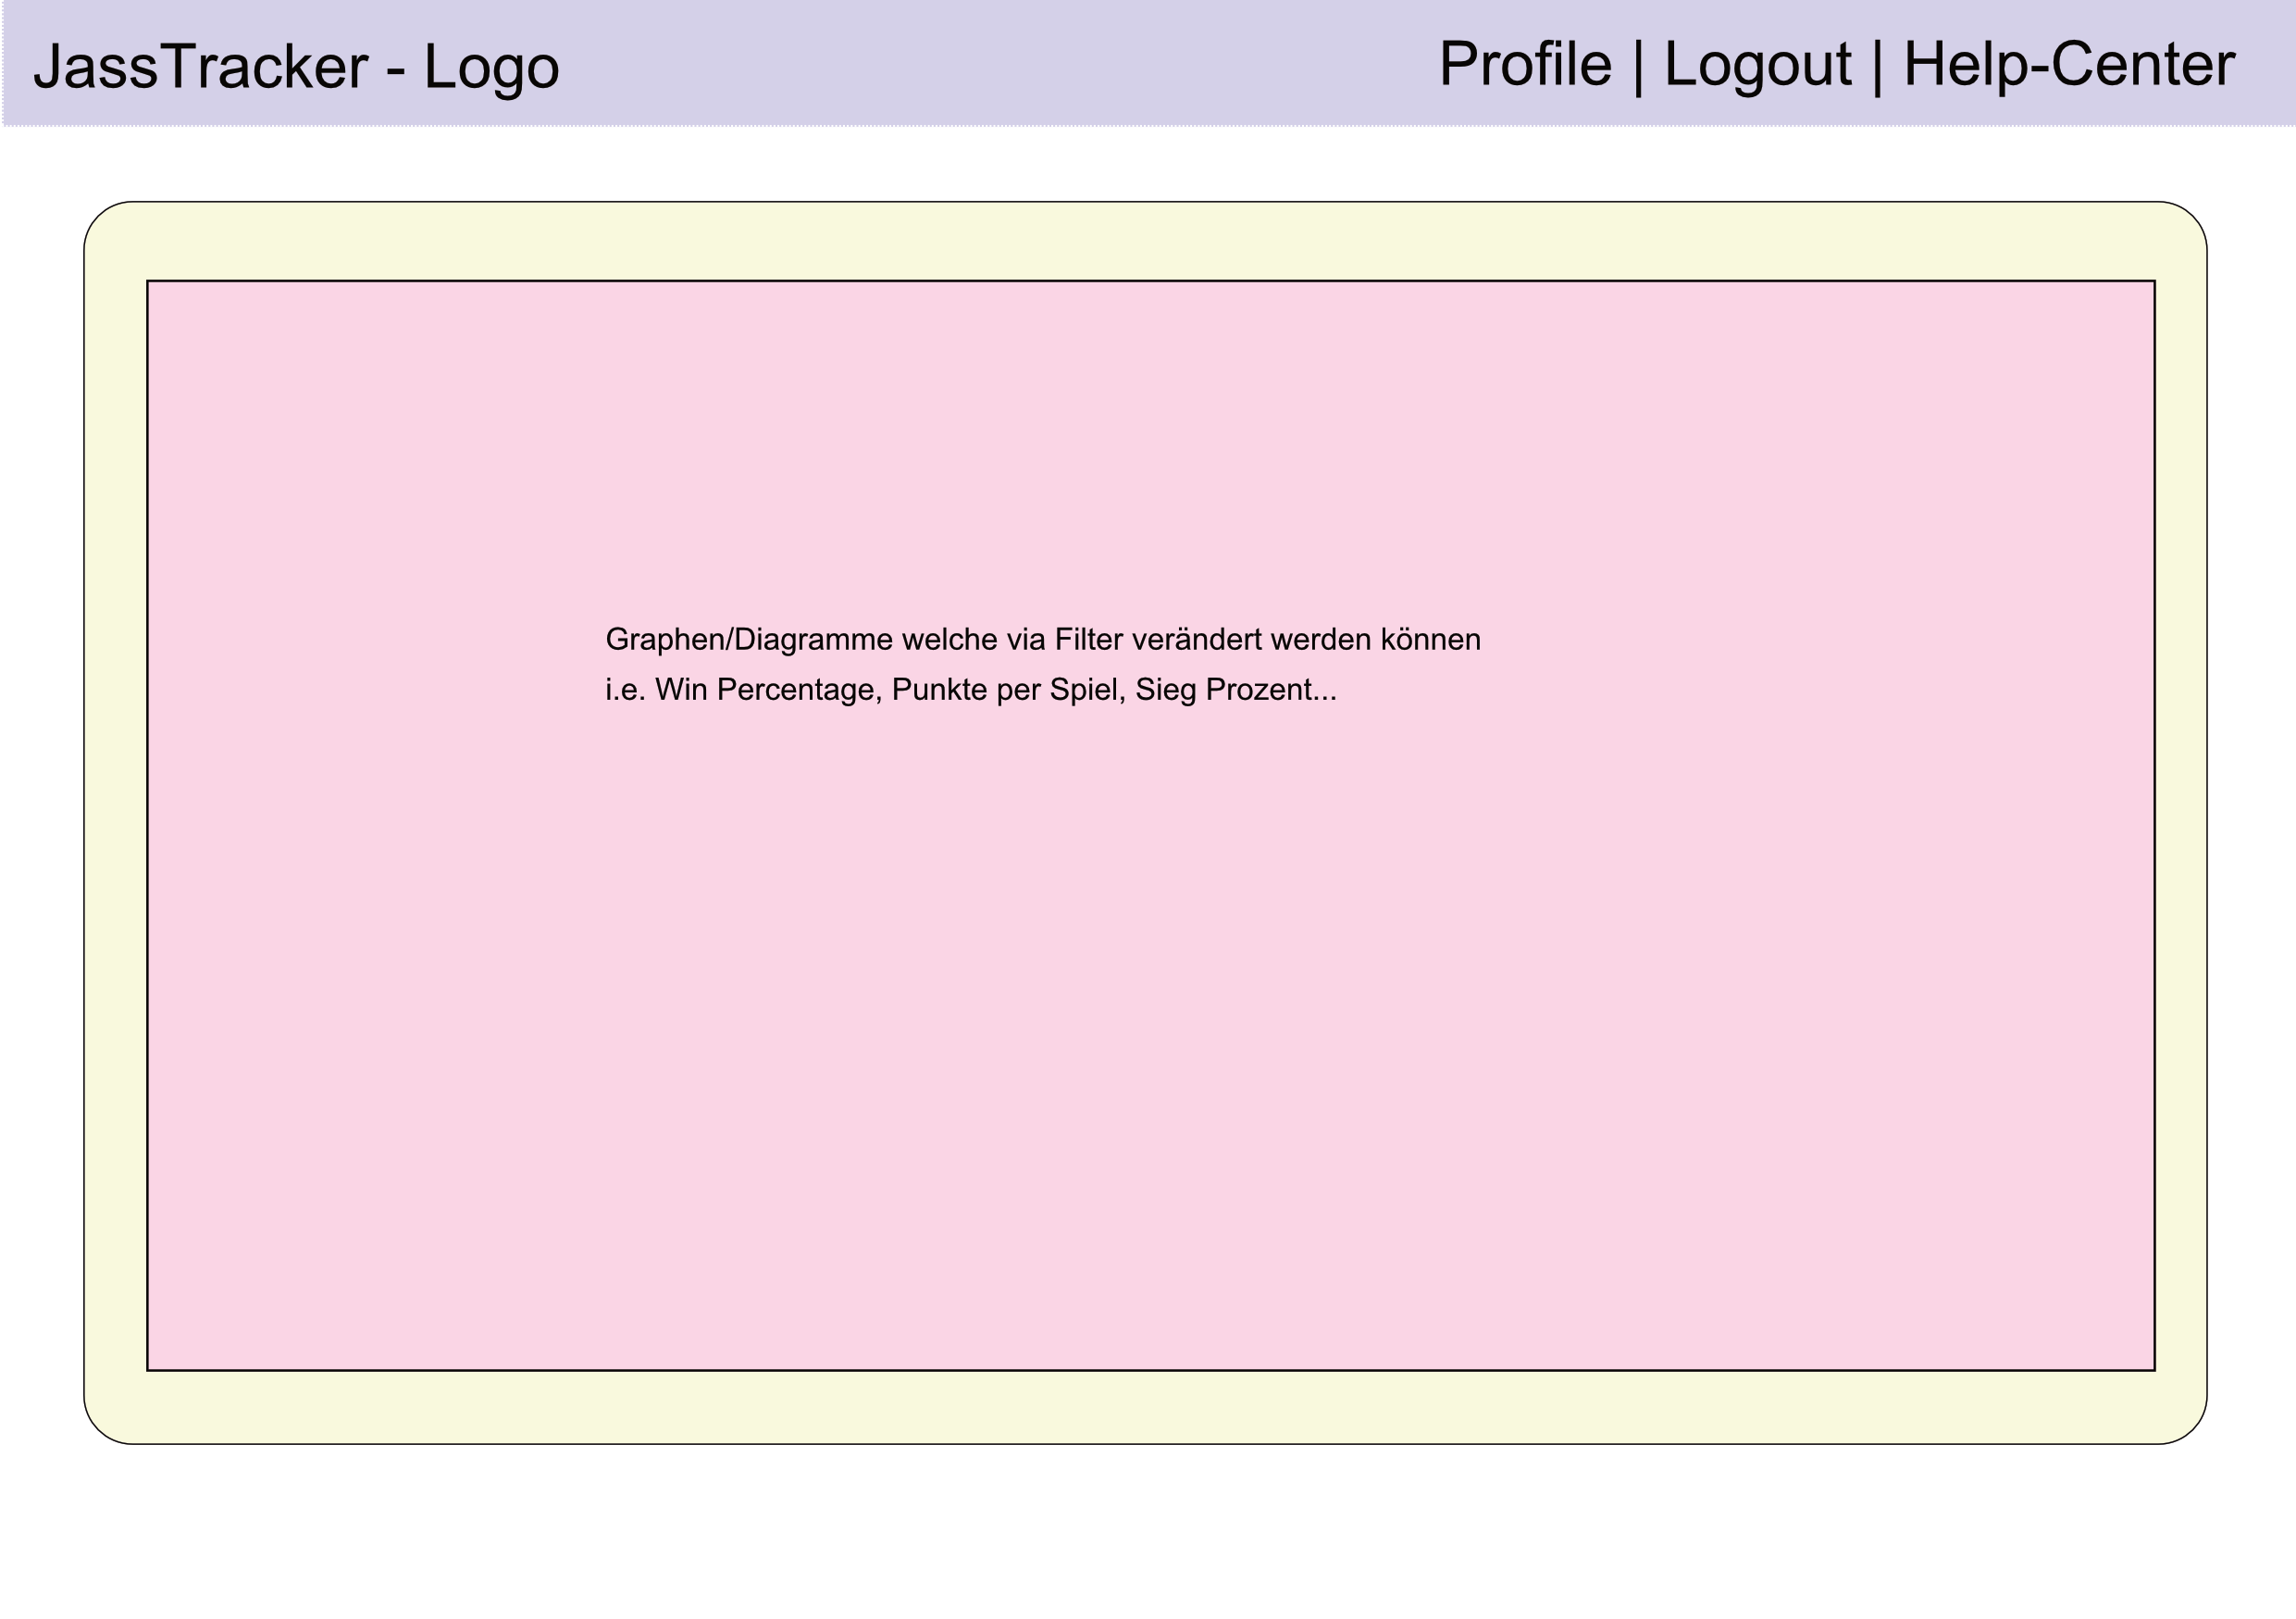
\includegraphics[height=10cm, width=\textwidth]{resources/mockups/mockup-player-stats.png}